\subsection{External Interface Requirements}

\subsubsection{User Interfaces}
The system allows users to interact with itself through two user interfaces:
\begin{itemize}
    \item[] \textbf{Web Application:} Accessible from a desktop or mobile web browser, it offers access to the system's functionalities, including user authentication, trip history visualization with individual trip statistics, the editor for creating and managing bike paths, search functionality for finding bike paths between origin and destination, and user profile management.
    \item[] \textbf{Mobile Application:} Designed for real time tracking of cycling activities with automatic obstacle detection through device sensors. It also provides access to all web application features optimized for mobile use.
\end{itemize}

\begin{figure}[H]
    \centering
    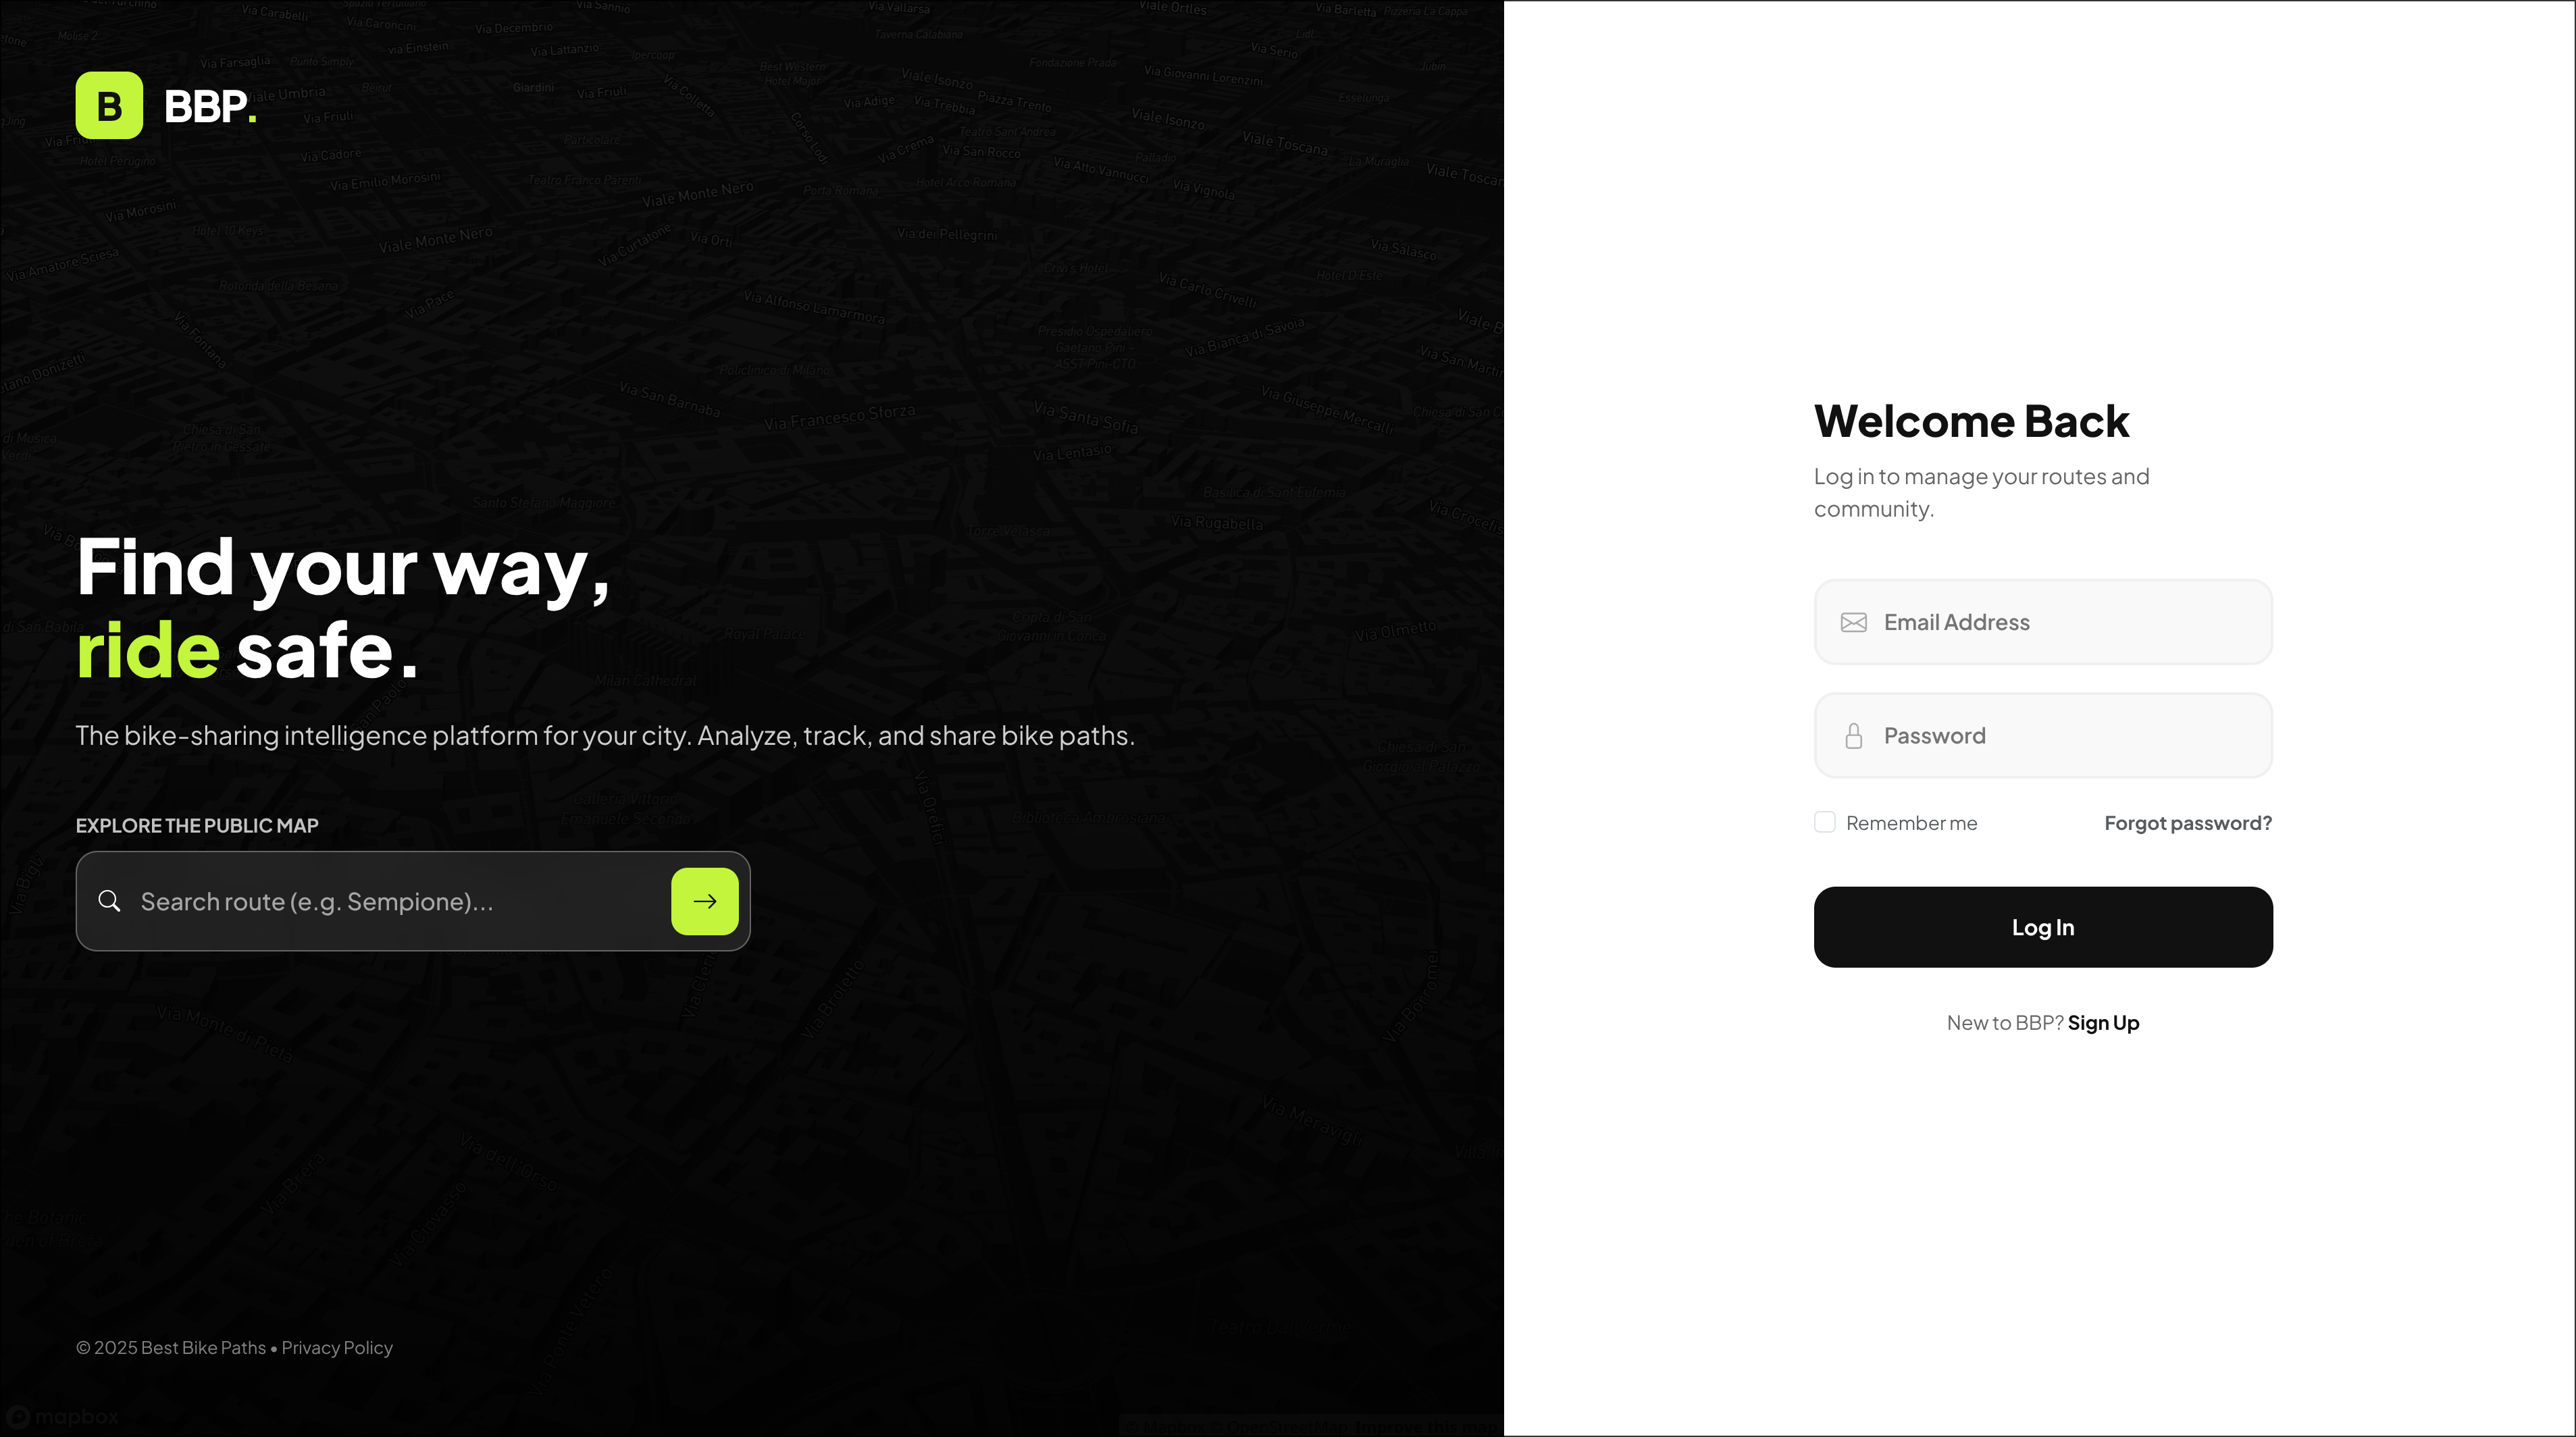
\includegraphics[width=\textwidth]{RASD/images/index.png}
    \caption{Homepage}
    \label{fig:index}
\end{figure}

\begin{figure}[H]
    \centering
    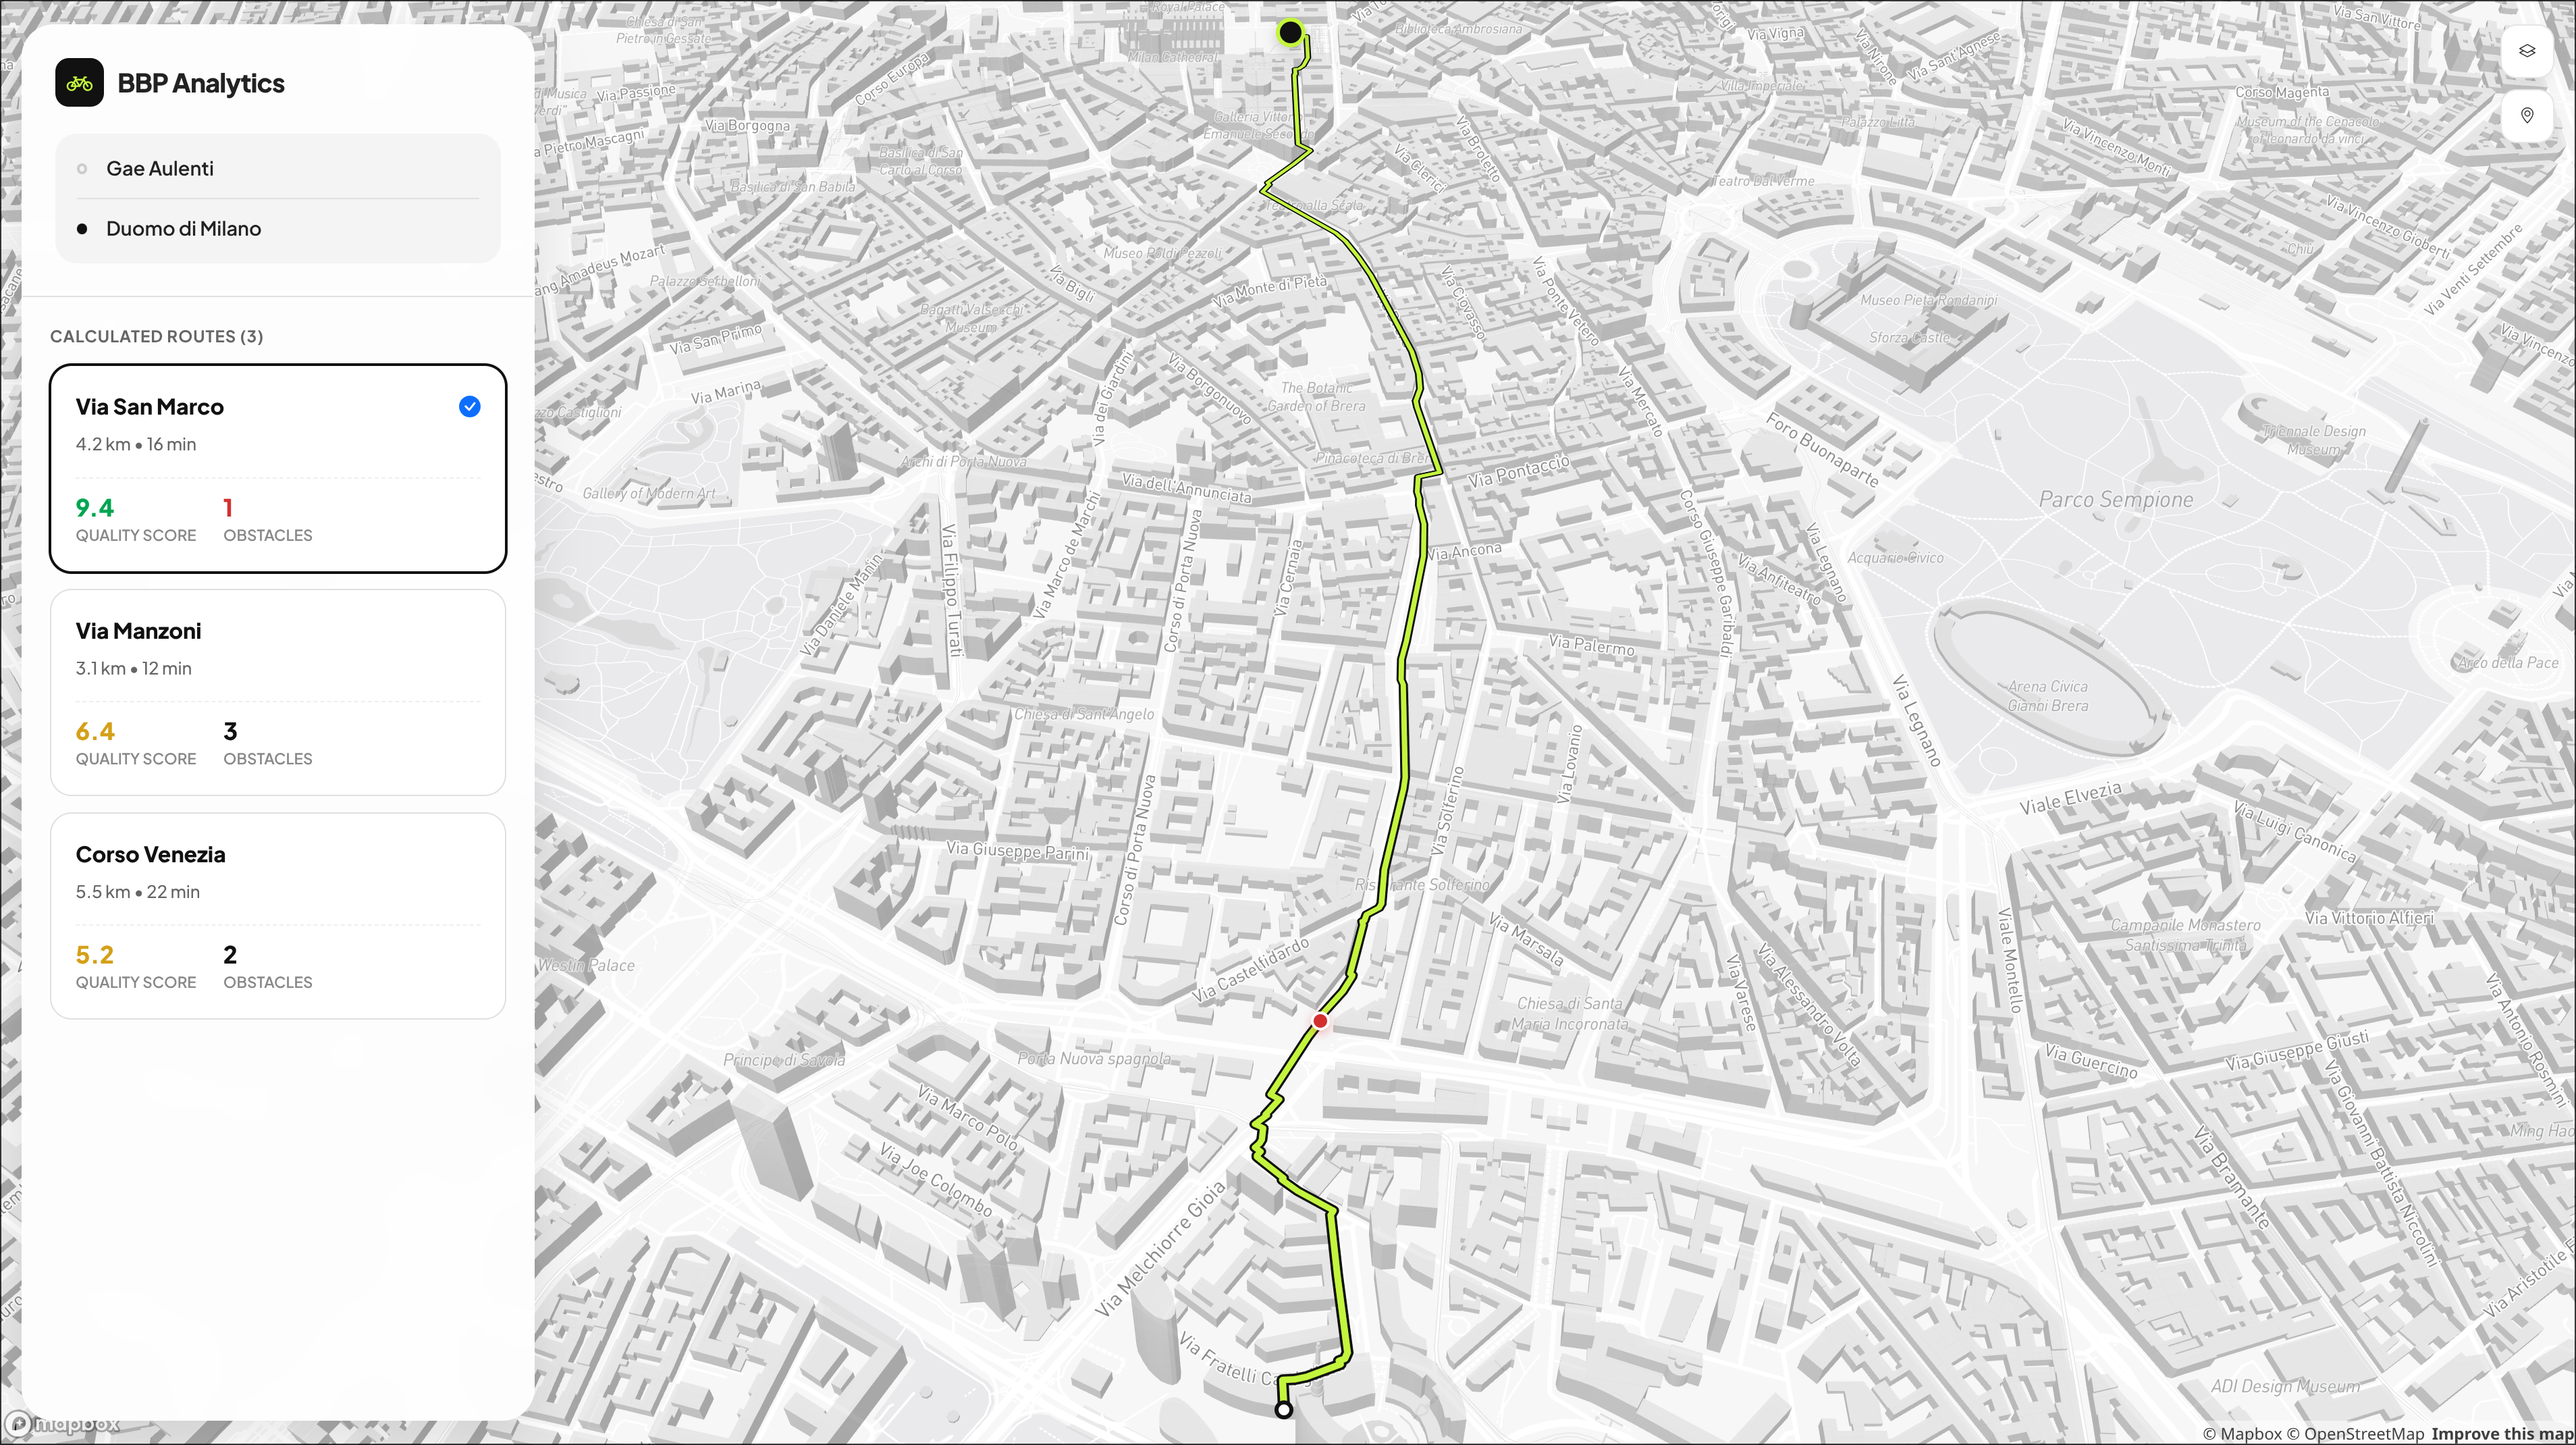
\includegraphics[width=\textwidth]{RASD/images/dashboard-desktop.png}
    \caption{Search results on desktop}
    \label{fig:dashboard-desktop}
\end{figure}

\begin{figure}[H]
    \centering
    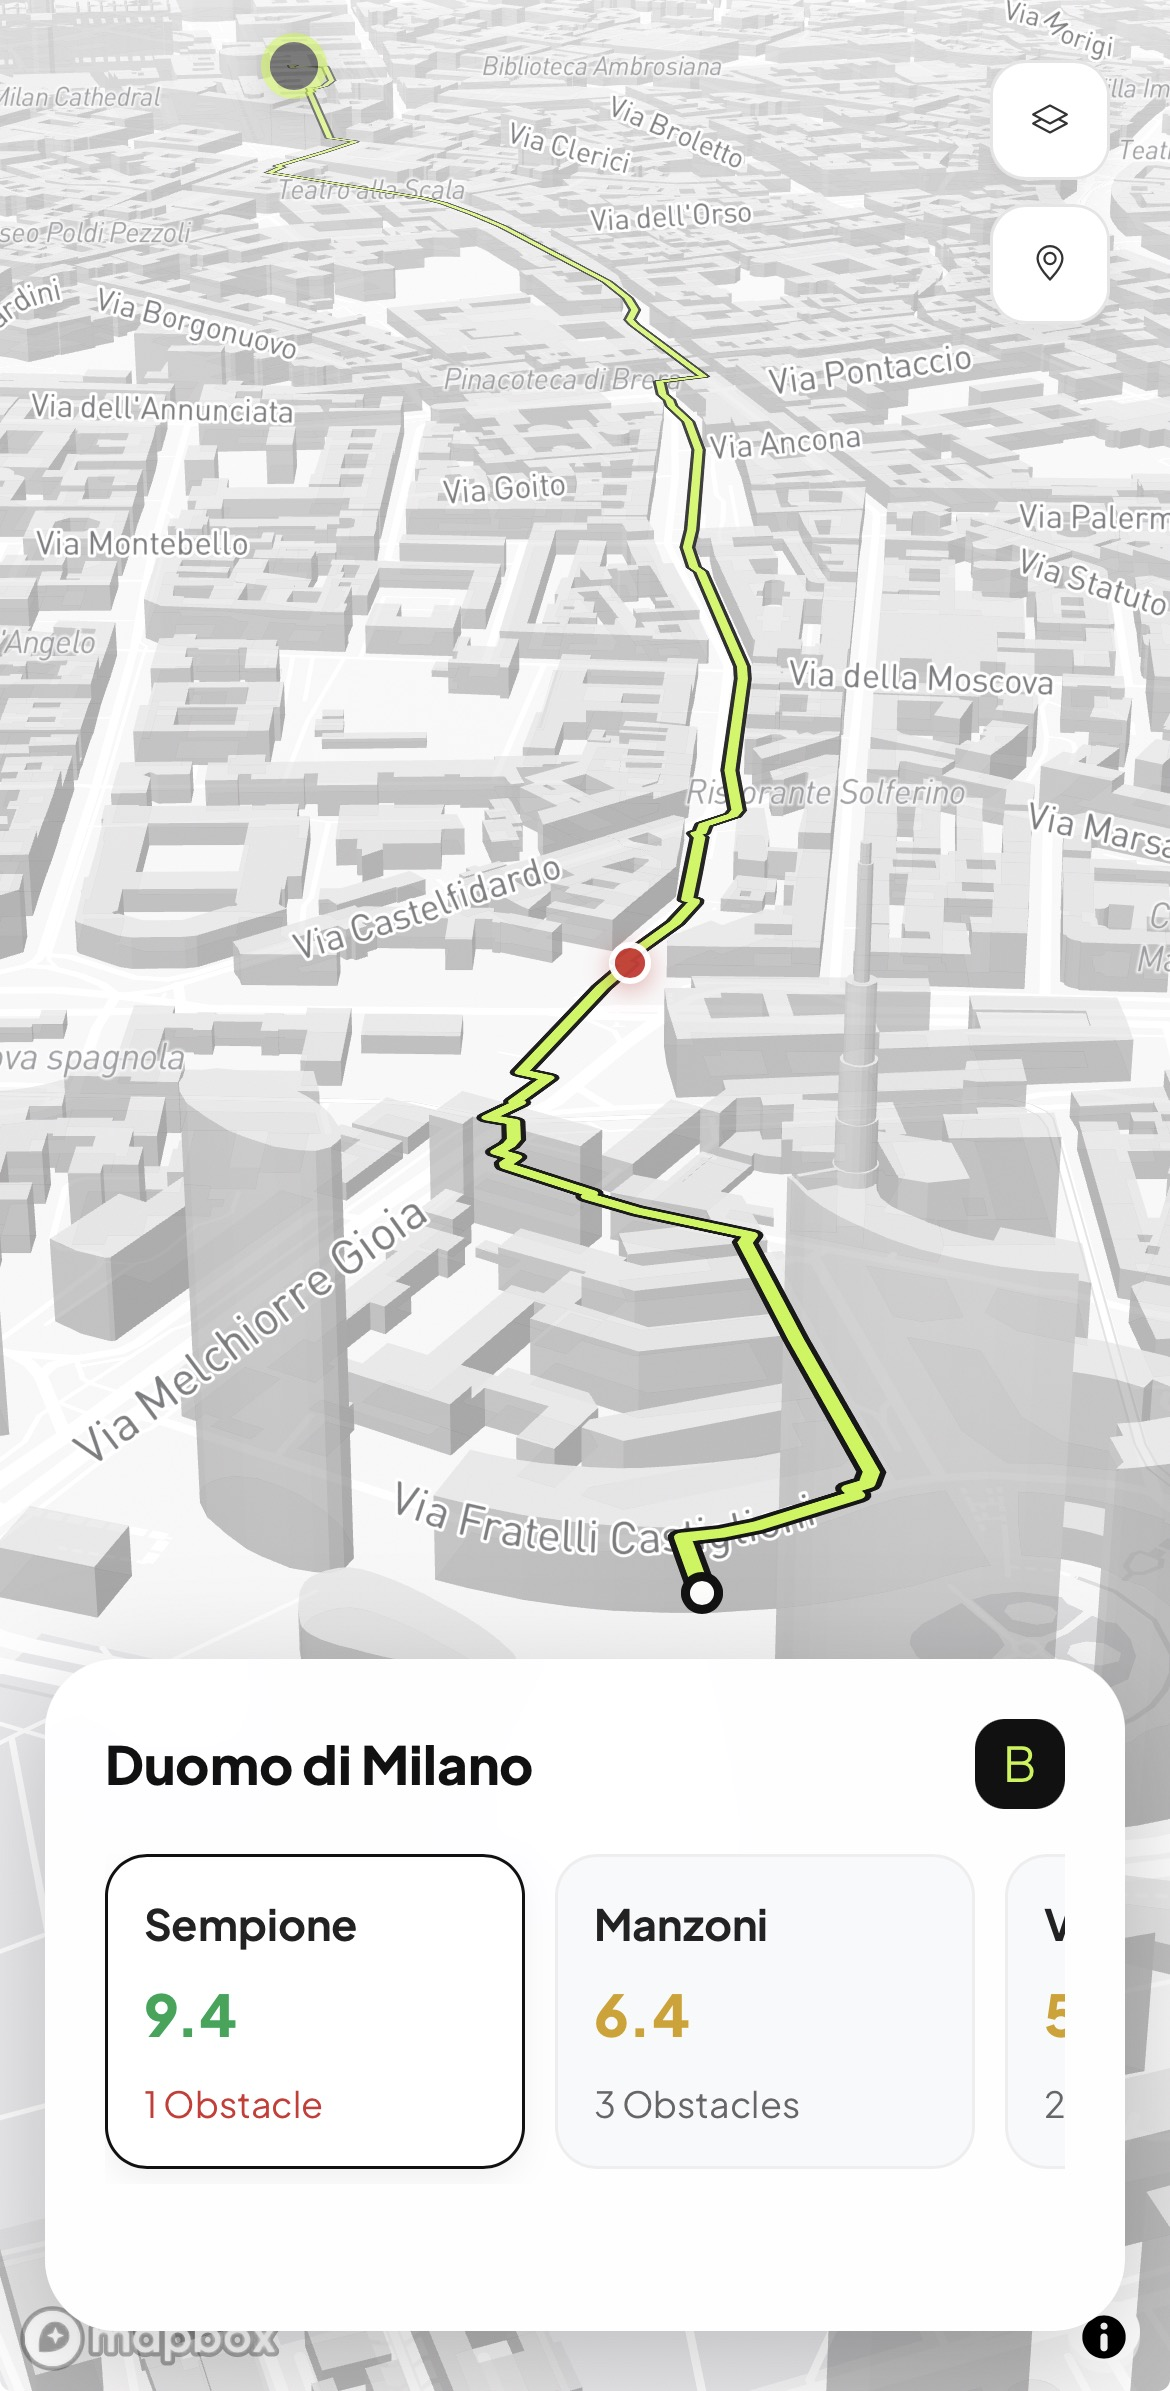
\includegraphics[width=\textwidth, height=0.85\textheight, keepaspectratio]{RASD/images/dashboard-mobile.png}
    \caption{Search results on mobile}
    \label{fig:dashboard-mobile}
\end{figure}

\begin{figure}[H]
    \centering
    \includegraphics[width=\textwidth]{RASD/images/my-path.png}
    \caption{A personal path}
    \label{fig:personal-path}
\end{figure}

\begin{figure}[H]
    \centering
    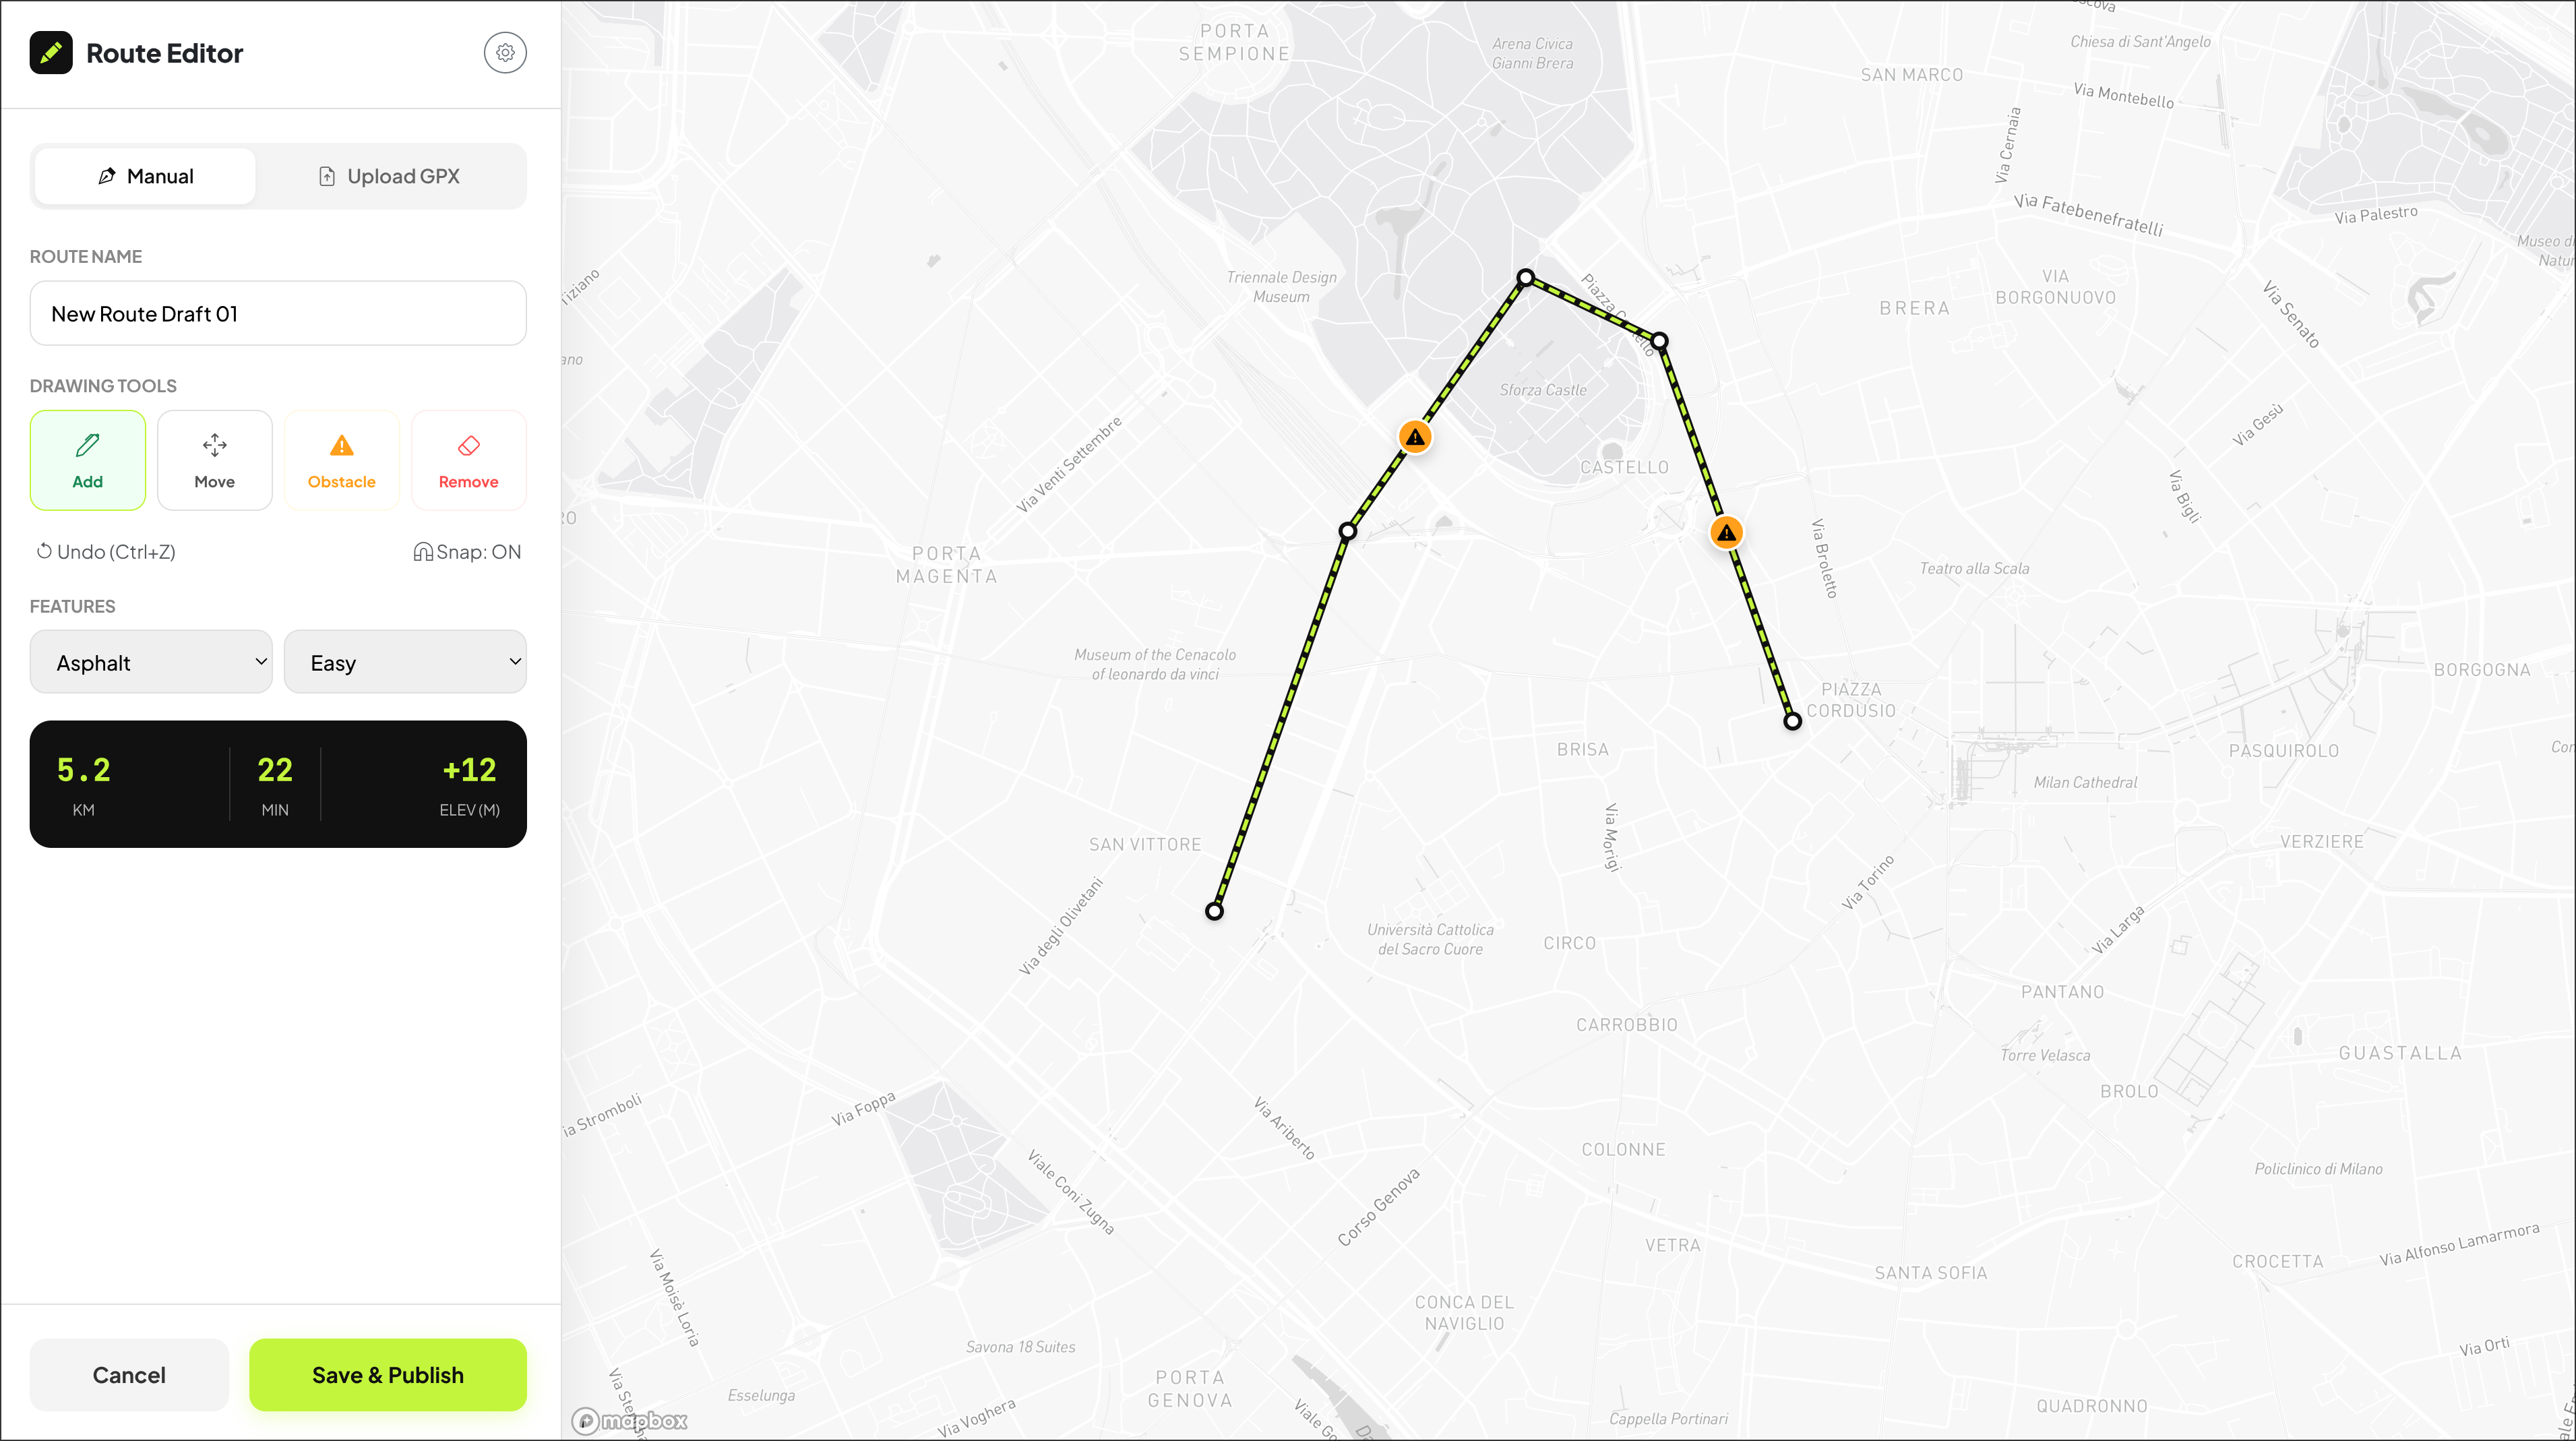
\includegraphics[width=\textwidth]{RASD/images/manual-insert.png}
    \caption{Manual insertion of a path}
    \label{fig:manual-insert}
\end{figure}

\begin{figure}[H]
    \centering
    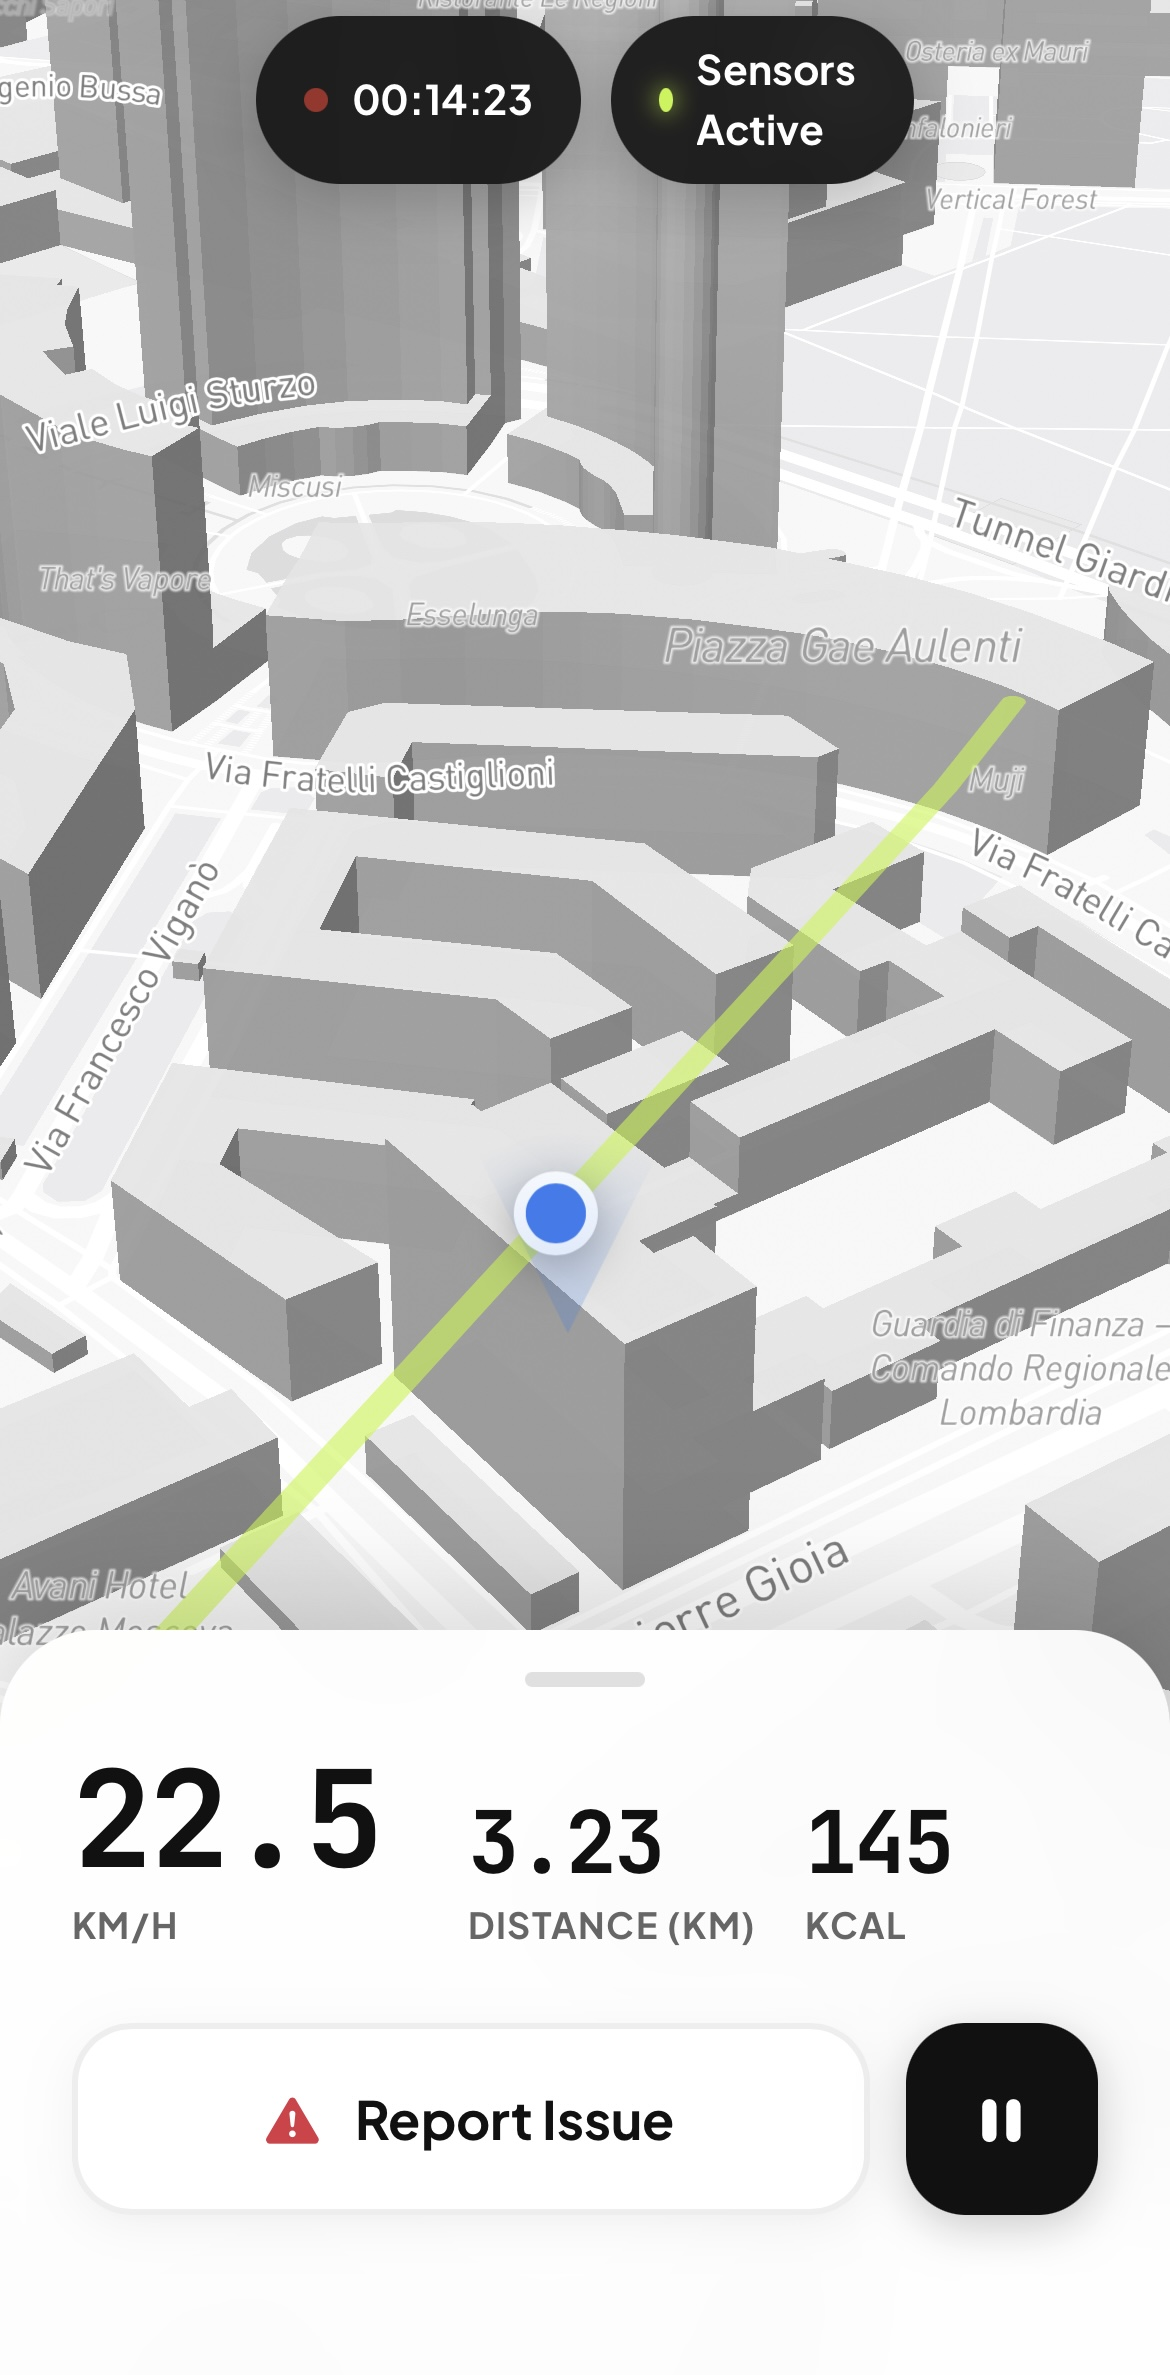
\includegraphics[width=\textwidth, height=0.85\textheight, keepaspectratio]{RASD/images/recording-trip.png}
    \caption{Mobile app while it's recording a trip}
    \label{fig:automatic-trip-record}
\end{figure}

\begin{figure}[H]
    \centering
    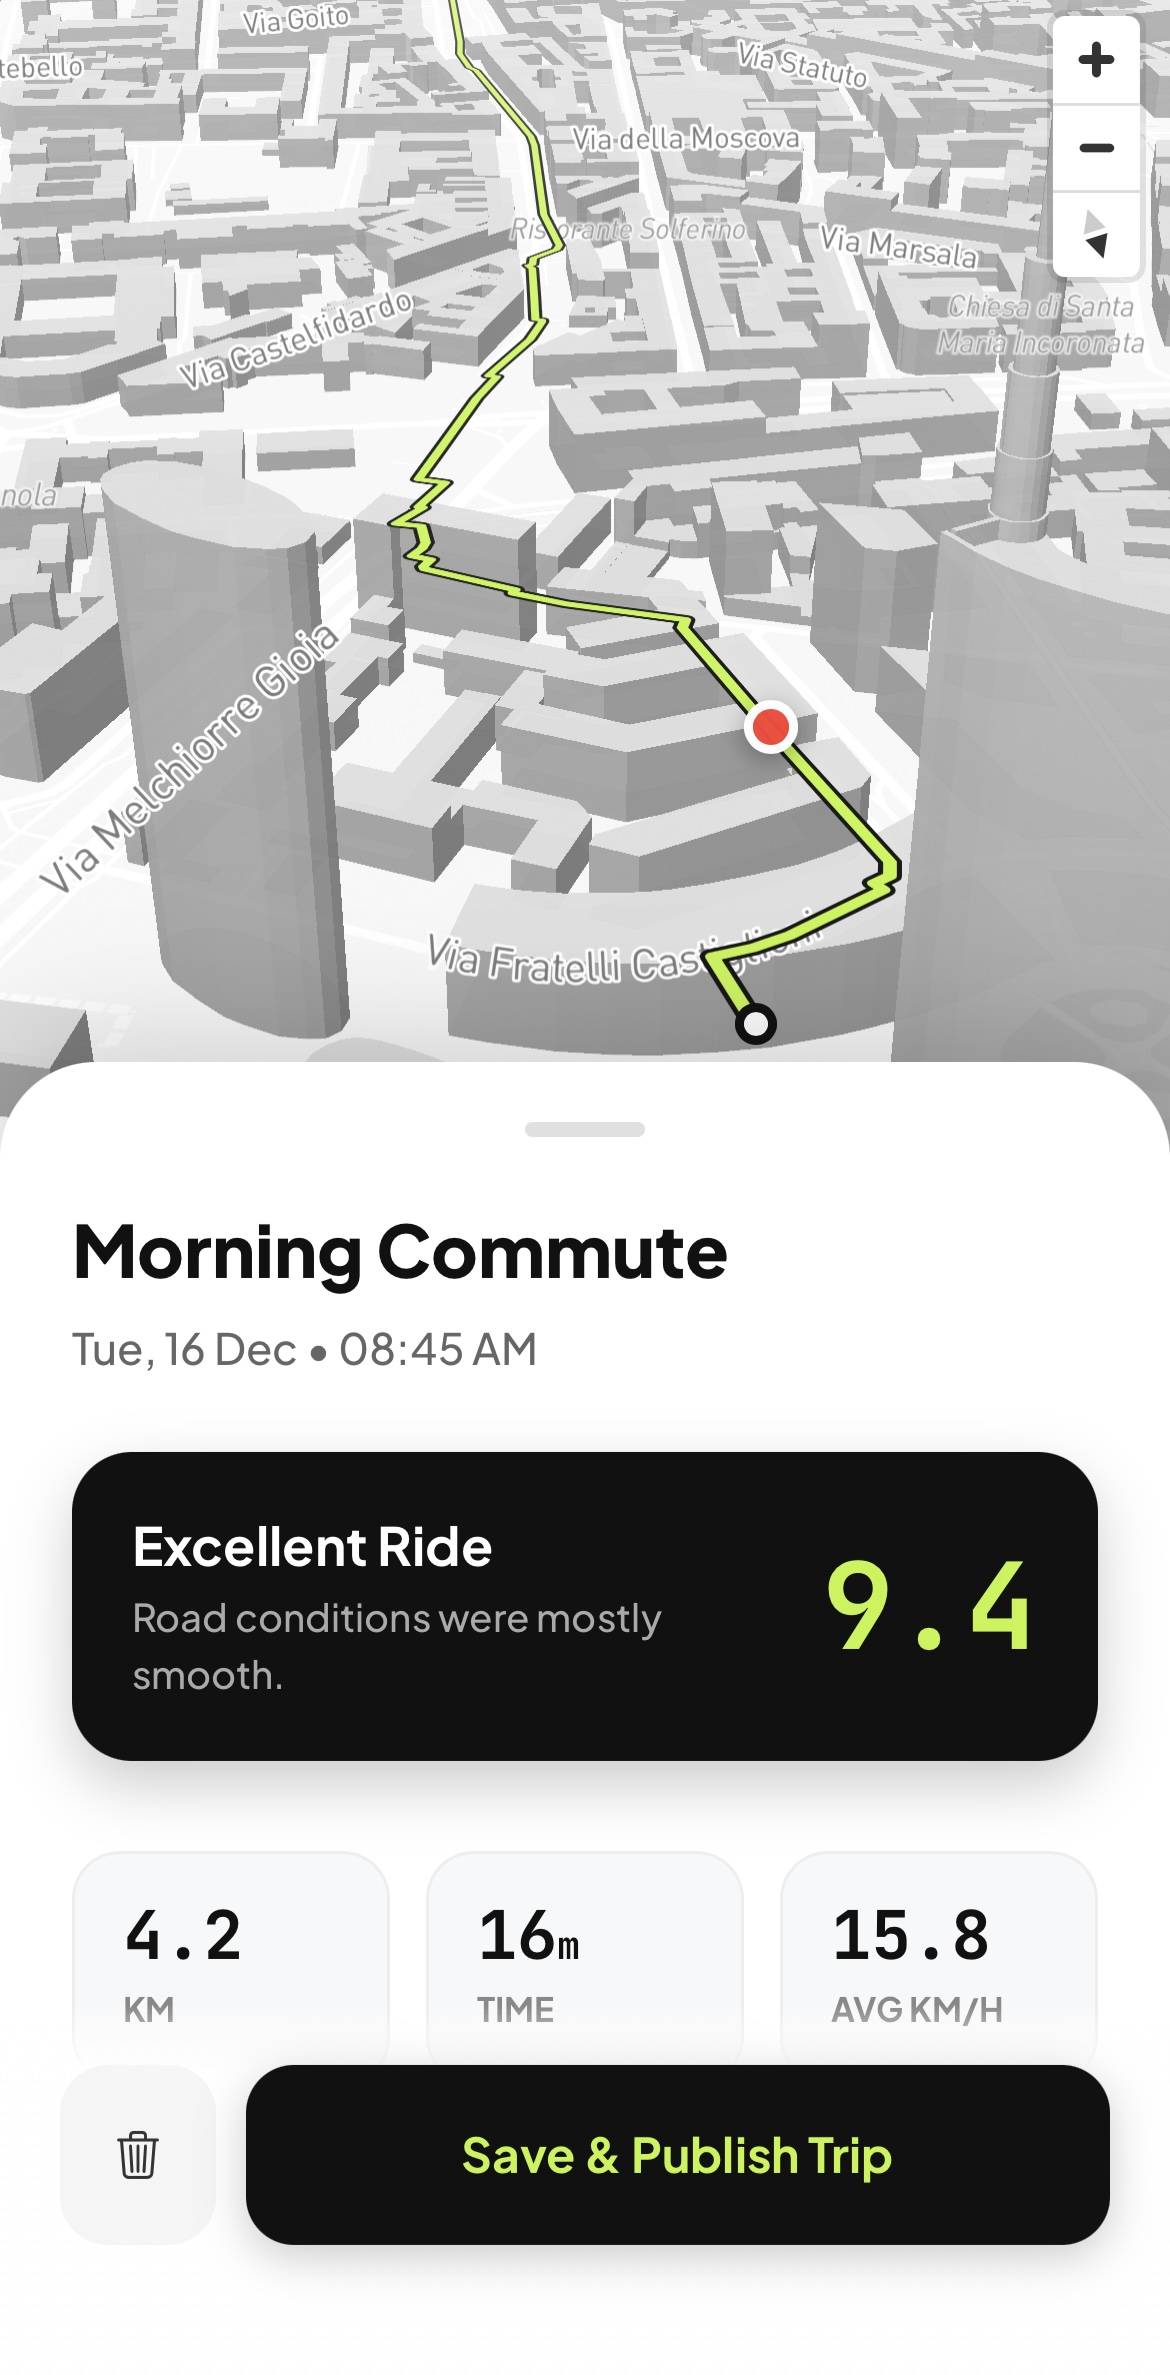
\includegraphics[width=\textwidth, height=0.85\textheight, keepaspectratio]{RASD/images/validation-summary.PNG}
    \caption{Mobile app when it stops recording}
    \label{fig:validation-summary}
\end{figure}

\begin{figure}[H]
    \centering
    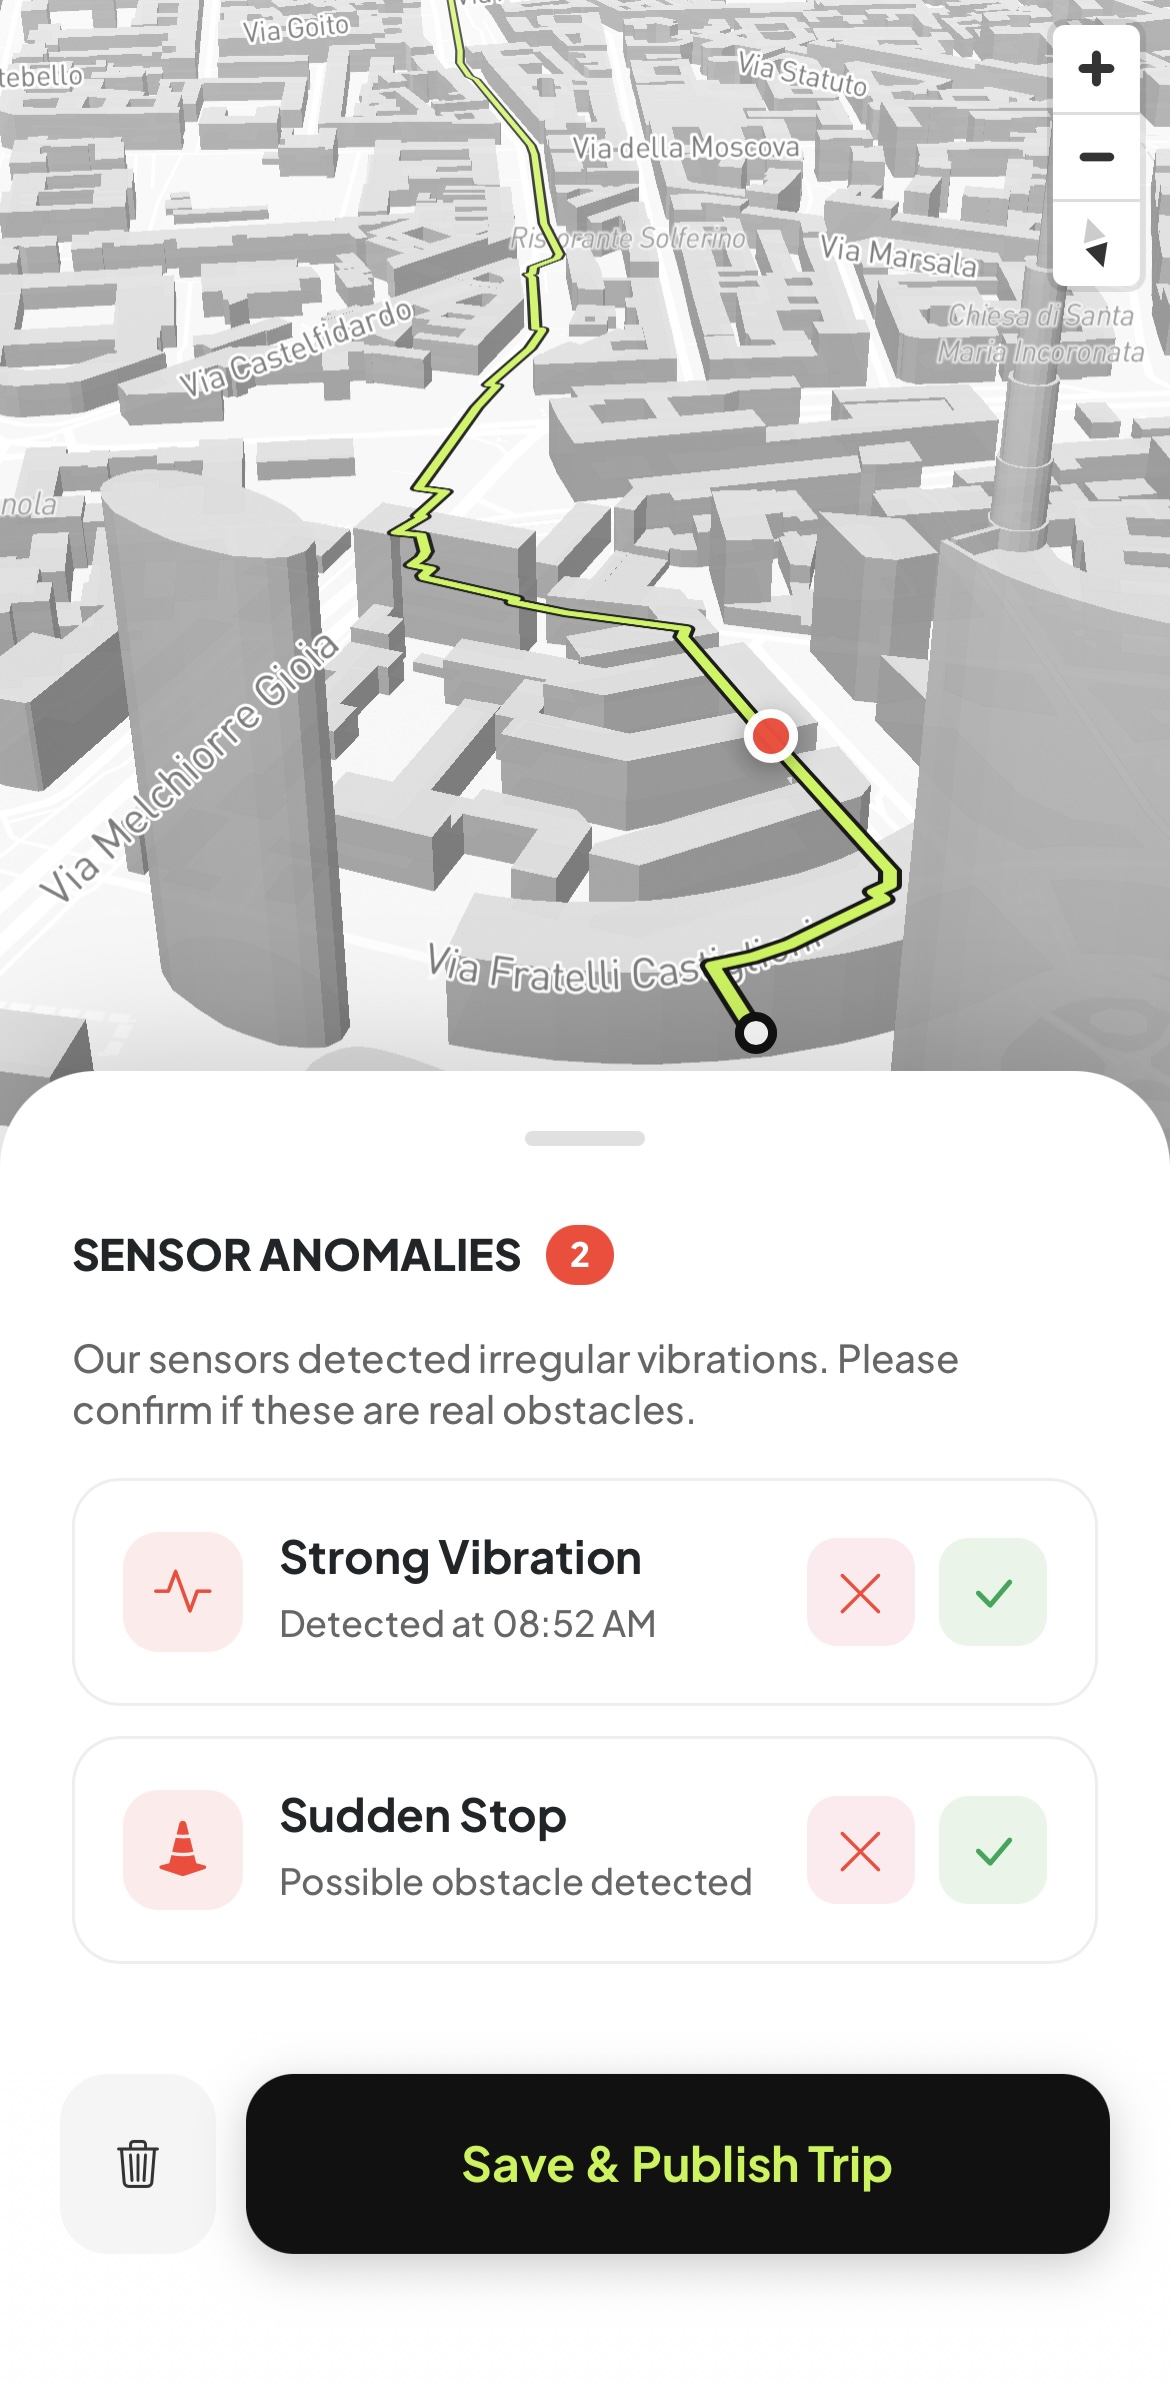
\includegraphics[width=\textwidth, height=0.85\textheight, keepaspectratio]{RASD/images/validation-detected.png}
    \caption{Mobile app when it's asking for validation of detected obstacles}
    \label{fig:validation-detected}
\end{figure}

\clearpage

\subsubsection{Hardware Interfaces}
The mobile app requires several hardware components of users' mobile phones to enable GPS tracking and obstacle detection:
\begin{itemize}
    \item[] \textbf{GPS:} Used to track geographical location in real time, calculate the average speed, and record obstacle coordinates.
    \item[] \textbf{Accelerometer and Gyroscope:} Used by the mobile application to detect significant vertical shocks and sudden changes in movement, identifying potential road surface anomalies (for example potholes) during automatic tracking.
\end{itemize}

\subsubsection{Software Interfaces}
The system uses API and external software components to provide its core functionalities:
\begin{itemize}
    \item[] \textbf{Map API:} Interface used for three critical functionalities:
    \begin{itemize}
        \item[] \textit{Geocoding API:} Used to convert the addresses submitted by the users to geographical coordinates.
        \item[] \textit{Directions API:} Used to calculate the optimal bike path between two points and determine the exact distance.
        \item[] \textit{Maps SDK:} Used to visualize the maps on the user interface.
    \end{itemize}
    \item[] \textbf{Weather API:} Interface used to get historical weather data based on time, date and location.
\end{itemize}

\subsubsection{Communication Interfaces}
The system utilizes the following protocols for data transfers:
\begin{itemize}
    \item[] \textbf{REST on HTTPS:} All client-server communications take place via RESTful APIs protected by TLS/SSL encryption.
    \item[] \textbf{JSON:} Standard format used for the payload of API requests and responses.
    \item[] \textbf{JWT (JSON Web Token):} Used in the HTTP Authorization header to handle secure and stateless user authentication.
\end{itemize}

\subsection{Functional Requirements}
This section lists the functional requirements of the BBP system, grouped by functional area, and describes the main Use Cases.

\subsubsection{List of Functional Requirements}

\paragraph{Authentication \& User Profile}
\begin{itemize}
    \item[] \textbf{[R1]} The system allows users to register with a valid email address and a password.
    \item[] \textbf{[R2]} The system allows registered users to log in and get a session token.
    \item[] \textbf{[R3]} The system allows registered users to log out.
    \item[] \textbf{[R4]} The system allows registered users to edit their accounts or delete them.
\end{itemize}

\paragraph{Trip Management}
\begin{itemize}
    \item[] \textbf{[R5]} The system allows registered users to manually insert a trip specifying the starting point, the destination point, the starting time, the time of arrival, and the streets composing the route.
    \item[] \textbf{[R6]} The system has to automatically calculate the total distance and the average speed of a manually inserted trip.
    \item[] \textbf{[R7]} The system has to enrich users' trips with weather data (temperature, weather conditions, wind speed), if available.
    \item[] \textbf{[R8]} The system allows registered users to automatically track their trips in real time.
\item[] \textbf{[R9]} The system allows registered users to view their trip history with individual trip statistics (distance, speed, duration, weather) and map visualization.
\item[] \textbf{[R10]} The system allows registered users to delete their trips.
\end{itemize}

\paragraph{Bike Path Management}
\begin{itemize}
    \item[] \textbf{[R11]} The system allows registered users to create new bike paths by specifying origin, destination, and the streets composing the route.
    \item[] \textbf{[R12]} The system allows registered users to automatically record bike paths through GPS tracking and sensor data, with user validation before publishing.
    \item[] \textbf{[R13]} The system calculates the exact geometry and length of the path using an external routing service.
    \item[] \textbf{[R14]} The system allows registered users to add obstacles to a bike path, specifying the type and severity.
    \item[] \textbf{[R15]} The system validates that the reported obstacles are within a specific buffer distance from the path.
    \item[] \textbf{[R16]} The system automatically calculates a quality score for each bike path, based on its maintenance status and present obstacles.
    \item[] \textbf{[R17]} The system allows the creator of a bike path to manage its visibility (private or public) and maintenance status.
    \item[] \textbf{[R18]} The system allows the creator of a bike path to delete it.
\end{itemize} 

\paragraph{Search \& Exploration}
\begin{itemize}
    \item[] \textbf{[R19]} The system allows any user (both registered and non registered) to search for public bike paths between an origin and a destination.
    \item[] \textbf{[R20]} The system shows search results sorted by descending quality score.
\end{itemize}

\paragraph{Collaborative Maintenance}
\begin{itemize}
    \item[] \textbf{[R21]} The system allows registered users to report new obstacles on existing public bike paths.
    \item[] \textbf{[R22]} The system allows registered users to update existing obstacles (type, severity, active status).
    \item[] \textbf{[R23]} The system automatically recalculates the quality score of a bike path each time its obstacles are updated.
\end{itemize}

\subsubsection{Use Cases}

The following tables describe the main use cases of the system.

\begin{table}[H]
    \centering
    \begin{tabular}{|p{4cm}|p{10cm}|}
        \hline
        Title & \textbf{Manual Trip Insertion} \\
        \hline
        Actors & Registered User, The System, External Routing Service, External Weather Service \\
        \hline
        Entry Condition & The user logs in and goes to "Add Trip" section. \\
        \hline
        Event Flow & 
        (a) The user inserts the starting address, the destination address, the streets composing the route, the starting time and the arrival time. \newline
        (b) The system calls an external routing service to calculate the exact route geometry and distance, and calculates the duration from the provided times. \newline
        (c) If available, the system retrieves historical weather data and enriches the trip. \newline
        (d) The system saves the trip to the user profile. \newline
        (e) The system confirms the successful save to the user. \\
        \hline
        Exit Condition & The trip with all data is logged in the user's trip history. \\
        \hline
        Exception & 
        \\
        \hline
    \end{tabular}
    \caption{[UC1] Manual Trip Insertion}
    \label{tab:uc1}
\end{table}

\begin{table}[H]
    \centering
    \begin{tabular}{|p{4cm}|p{10cm}|}
        \hline
        Title & \textbf{Creation of a Public Bike Path} \\
        \hline
        Actors & Registered User, The System, External Routing Service \\
        \hline
        Entry Condition & The user logs in and goes to "Create Bike Path" section. \\
        \hline
        Event Flow & 
        (a) The user defines the waypoints of the bike path on the map. \newline
        (b) The system shows a route preview. \newline
        (c) The user adds metadata (status and description) and obstacles, if any. \newline
        (d) The user chooses between making the bike path public or private and submits. \newline
        (e) The system calculates the exact geometry of the path using an external routing service. \newline
        (f) The system validates that all obstacles are within a buffer distance from the path. \newline
        (g) The system calculates the quality score of the path and saves it. \newline
        (h) The system confirms the path creation to the user. \\
        \hline
        Exit Condition & The bike path has been created and made public or kept private. \\
        \hline
        Exception & 
        Validation failed: the system shows an error and prompts the user to correct invalid data. \\
        \hline
    \end{tabular}
    \caption{[UC2] Creation of a Public Bike Path}
    \label{tab:uc2}
\end{table}

\begin{table}[H]
    \centering
    \begin{tabular}{|p{4cm}|p{10cm}|}
        \hline
        Title & \textbf{Search of Bike Paths} \\
        \hline
        Actors & User (Registered or not registered), The System \\
        \hline
        Entry Condition & The user is on the "Bike Path Search Page". \\
        \hline
        Event Flow & 
        (a) The user enters the origin address and destination address. \newline
        (b) The system finds all public bike paths within a geographic radius. \newline
        (c) The system sorts the results by descending quality score. \newline
        (d) The system displays the ranked list of paths. \newline
        (e) The user selects a specific path. \newline
        (f) The system shows the full path details (route, obstacles, status). \\
        \hline
        Exit Condition & The user views the complete details of a selected bike path. \\
        \hline
        Exception & 
        Invalid addresses: the system prompts the user to correct the input. \\
        \hline
    \end{tabular}
    \caption{[UC3]: Search of Bike Paths}
    \label{tab:uc3}
\end{table}

\begin{table}[H]
    \centering
    \begin{tabular}{|p{4cm}|p{10cm}|}
        \hline
        Title & \textbf{Obstacle Reporting on Bike Path} \\
        \hline
        Actors & Registered User, The System \\
        \hline
        Entry Condition & The user is viewing the details of an existing public bike path. \\
        \hline
        Event Flow & 
        (a) The user selects "Report Issue". \newline
        (b) The user submits obstacle details (location, type, severity). \newline
        (c) The system validates the geographic coherence with the bike path. \newline
        (d) The system saves the new obstacle. \newline
        (e) The system recalculates the bike path quality score. \newline
        (f) The system broadcasts the update to other viewers. \newline
        (g) The system confirms the report was added. \\
        \hline
        Exit Condition & The bike path is updated with the new obstacle and the new score. \\
        \hline
        Exception & 
        Invalid obstacle location: the system shows an error message. \\
        \hline
    \end{tabular}
    \caption{[UC4] Obstacle Reporting on Bike Path}
    \label{tab:uc4}
\end{table}

\begin{table}[H]
    \centering
    \begin{tabular}{|p{4cm}|p{10cm}|}
        \hline
        Title & \textbf{Automatic Tracking} \\
        \hline
        Actors & Registered User, Mobile App, BBP Platform \\
        \hline
        Entry Condition & GPS is enabled and the app is open. \\
        \hline
        Event Flow & 
        (a) The app detects a speed typical for cycling and starts recording. \newline
        (b) During the ride, the app continuously records GPS coordinates and sensor data (accelerometer, gyroscope). \newline
        (c) If anomalies are detected, the app logs potential obstacles. \newline
        (d) The user stops riding and the app detects the prolonged stop. \newline
        (e) The app shows a summary with detected anomalies. \newline
        (f) The user confirms or discards the detected anomalies. \newline
        (g) The app uploads the trip data to the server. \newline
        (h) The system processes and saves the trip. \newline
        (i) The system acknowledges the upload. \newline
        (j) The app confirms the trip was saved successfully. \\
        \hline
        Exit Condition & The trip is saved and confirmed anomalies become reported obstacles. \\
        \hline
        Exception & Mobile phone battery dies. \\
        \hline
    \end{tabular}
    \caption{[UC5] Automatic Tracking}
    \label{tab:uc5}
\end{table}

\begin{table}[H]
    \centering
    \begin{tabular}{|p{4cm}|p{10cm}|}
        \hline
        Title & \textbf{User Registration} \\
        \hline
        Actors & Unregistered User, The System \\
        \hline
        Entry Condition & The user accesses the registration section. \\
        \hline
        Event Flow & 
        (a) The user submits username, email address, and password. \newline
        (b) The system validates input format and uniqueness. \newline
        (c) The system creates the new account with encrypted password. \newline
        (d) The system generates a session token. \newline
        (e) The system redirects the user to the dashboard. \\
        \hline
        Exit Condition & The user is registered and authenticated in the system. \\
        \hline
        Exception & 
        Invalid data: the system shows an error message. \\
        \hline
    \end{tabular}
    \caption{[UC6] User Registration}
    \label{tab:uc6}
\end{table}

\begin{table}[H]
    \centering
    \begin{tabular}{|p{4cm}|p{10cm}|}
        \hline
        Title & \textbf{User Login} \\
        \hline
        Actors & Registered User, The System \\
        \hline
        Entry Condition & The user opens the application or accesses the reserved area. \\
        \hline
        Event Flow & 
        (a) The user submits their email and password. \newline
        (b) The system verifies the credentials. \newline
        (c) The system generates an authentication token. \newline
        (d) The system grants access to the dashboard. \\
        \hline
        Exit Condition & The user is authenticated and can access protected features. \\
        \hline
        Exception & 
        Invalid credentials: the system shows an error message. \\
        \hline
    \end{tabular}
    \caption{[UC7] User Login}
    \label{tab:uc7}
\end{table}

\begin{table}[H]
    \centering
    \begin{tabular}{|p{4cm}|p{10cm}|}
        \hline
        Title & \textbf{Management of Created Bike Paths} \\
        \hline
        Actors & Creator User, The System \\
        \hline
        Entry Condition & The user opens the "My Bike Paths" section. \\
        \hline
        Event Flow & 
        (a) The system lists all bike paths created by the user. \newline
        (b) The user selects a bike path to manage. \newline
        (c.1) To modify: The user updates visibility (public/private) and/or maintenance status. The system saves changes and confirms. \newline
        (c.2) To delete: The user requests deletion. The system removes the bike path and associated data and confirms. \\
        \hline
        Exit Condition & The bike path is updated or removed from the system. \\
        \hline
        Exception & \\
        \hline
    \end{tabular}
    \caption{[UC8] Management of Created Bike Paths}
    \label{tab:uc8}
\end{table}

\begin{table}[H]
    \centering
    \begin{tabular}{|p{4cm}|p{10cm}|}
        \hline
        Title & \textbf{Trip History Visualization and Management} \\
        \hline
        Actors & Registered User, The System \\
        \hline
        Entry Condition & The user opens the "Trip Diary" section. \\
        \hline
        Event Flow & 
        (a) The system retrieves the user's trips. \newline
        (b) The system shows a list with individual trip statistics (distance, duration, speed, map) and weather conditions. \newline
        (c) Optionally, the user can apply filters or sorting criteria and the system updates the view. \newline
        (d) Optionally, the user can delete a specific trip. The system removes the trip data and confirms deletion. \\
        \hline
        Exit Condition & The user views their trip history with detailed statistics. \\
        \hline
        Exception & 
        No trips recorded: the system shows an empty list. \\
        \hline
    \end{tabular}
    \caption{[UC9] Trip History Visualization and Management}
    \label{tab:uc9}
\end{table}

\begin{table}[H]
    \centering
    \begin{tabular}{|p{4cm}|p{10cm}|}
        \hline
        Title & \textbf{User Profile Update} \\
        \hline
        Actors & Registered User, The System \\
        \hline
        Entry Condition & The user opens profile settings. \\
        \hline
        Event Flow & 
        (a) The user submits changes to their profile data. \newline
        (b) The system validates the new data. \newline
        (c) If valid: The system saves the changes and confirms update success. \newline
        (d) If invalid: The system shows an error message. \\
        \hline
        Exit Condition & The user profile is updated. \\
        \hline
        Exception & 
        Invalid email format or email already in use. \newline
        Username already exists. \newline
        Password does not meet security requirements. \\
        \hline
    \end{tabular}
    \caption{[UC10] User Profile Update}
    \label{tab:uc10}
\end{table}

\clearpage

\subsubsection{Sequence Diagrams}
The following sequence diagrams represent all the above Use Cases, they represent the interactions between the users and the system at a reasonable high level.

\begin{figure}[h!]
    \centering
    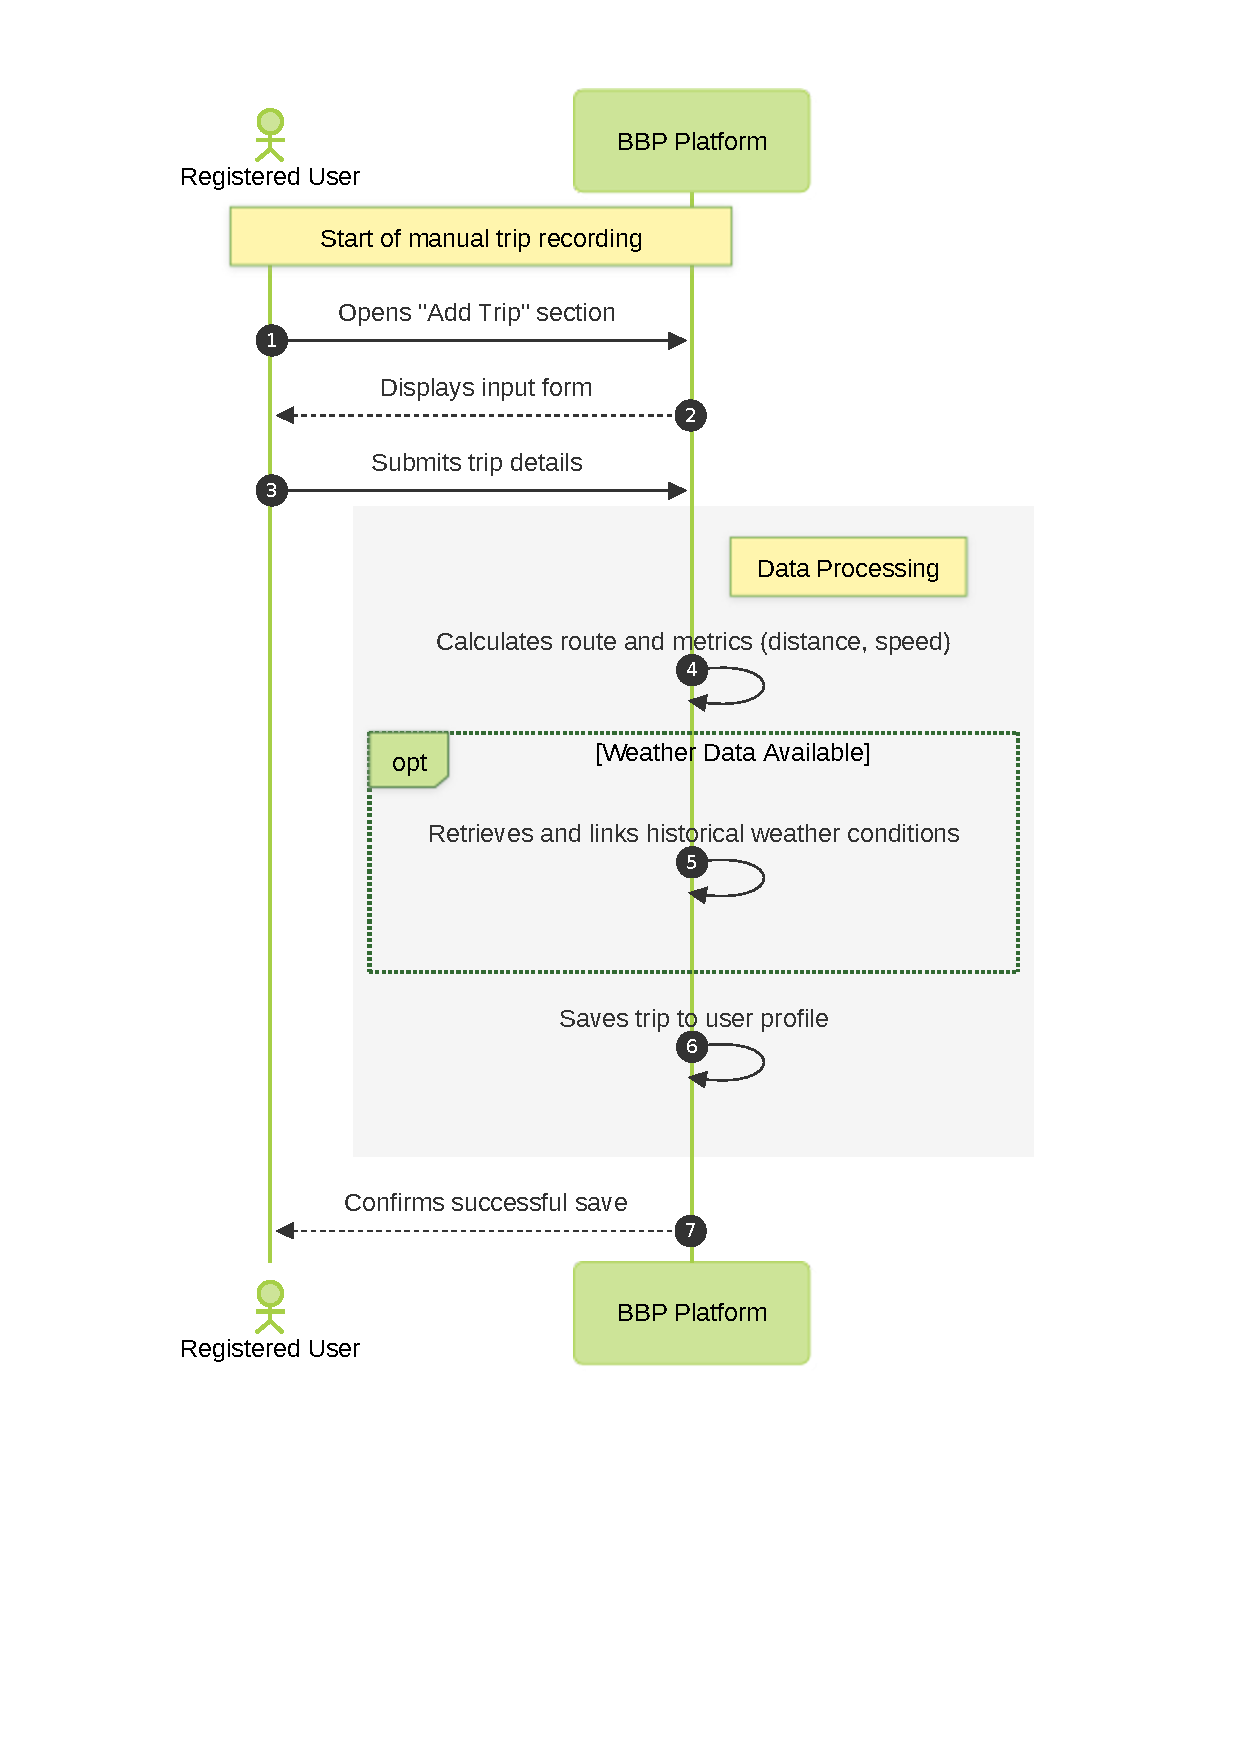
\includegraphics[height=0.7\textheight, keepaspectratio]{RASD/images/uc01.pdf}
    \caption{Manual Trip Insertion}
    \label{fig:uc1}
\end{figure}

\begin{figure}[h!]
    \centering
    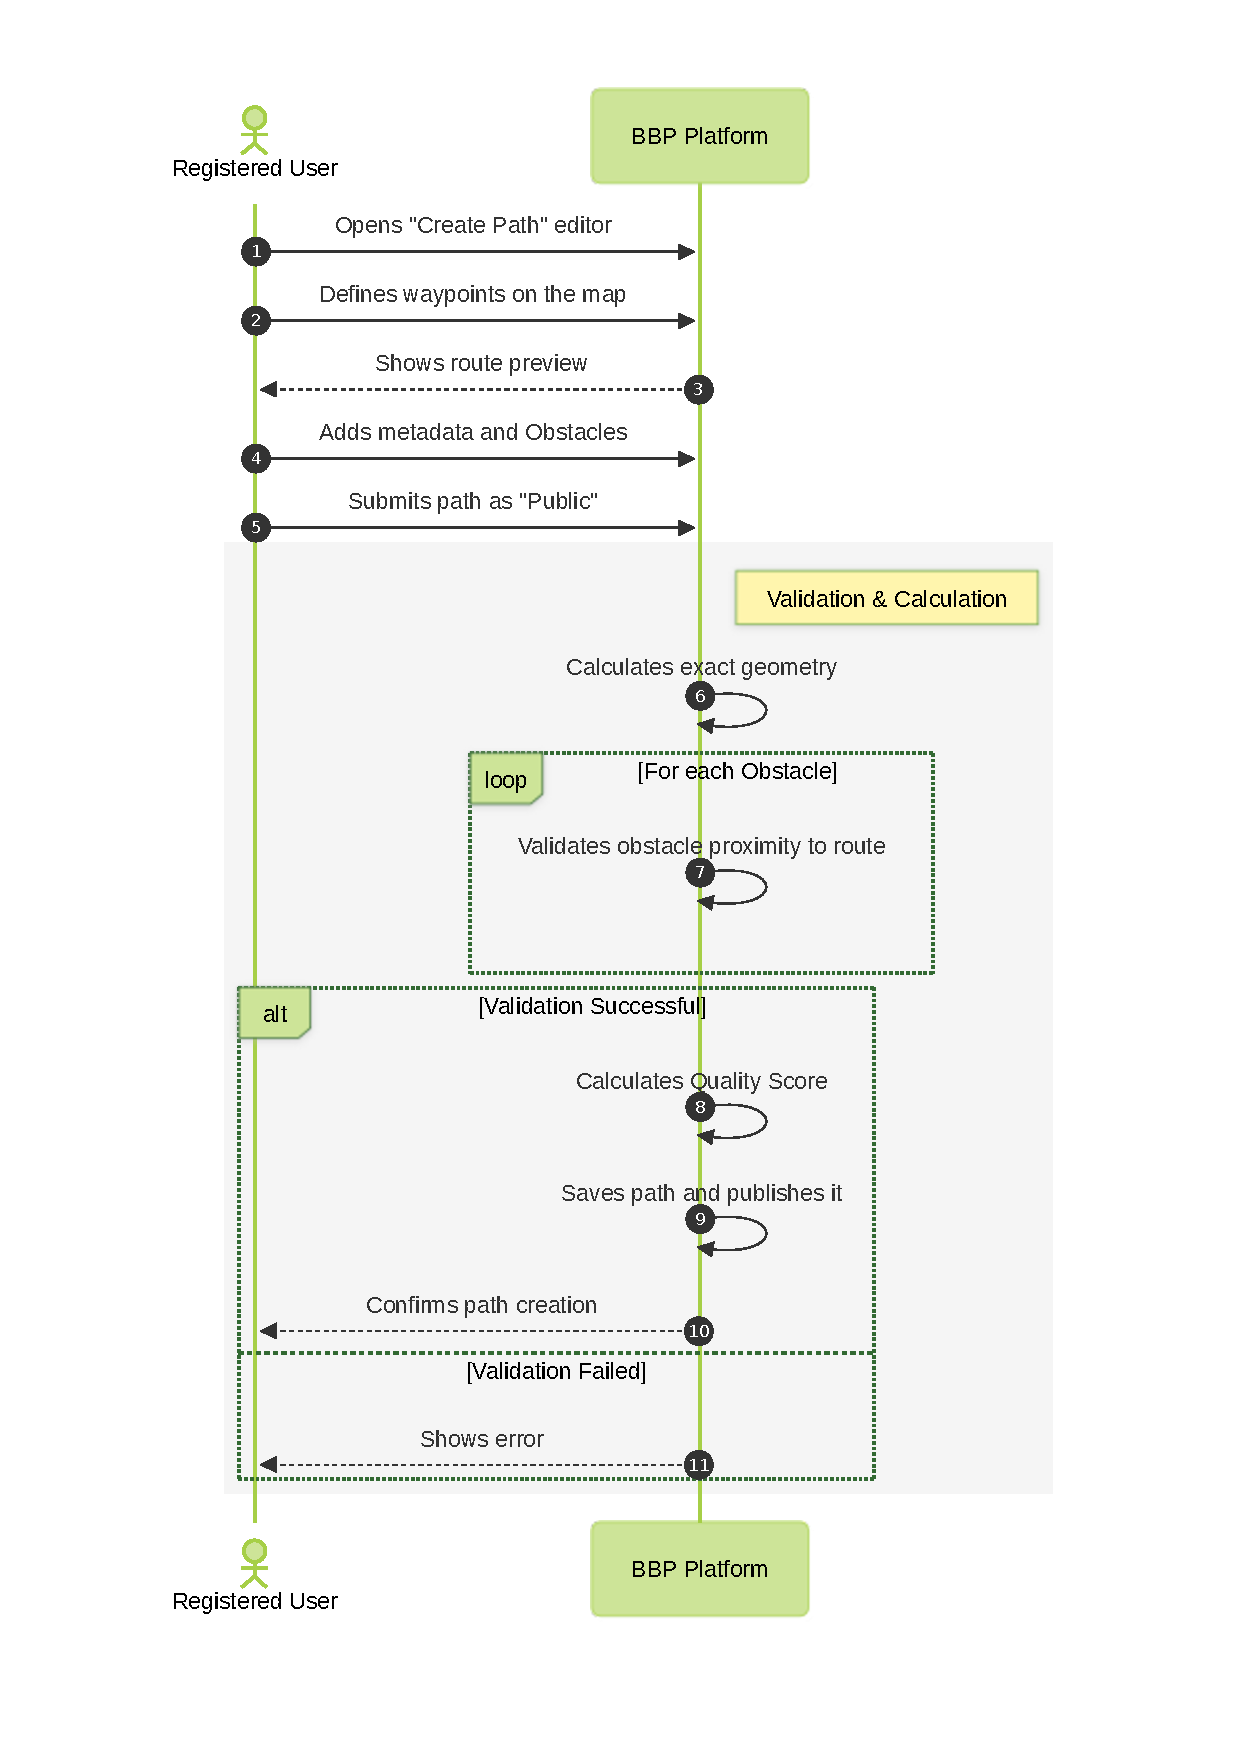
\includegraphics[width=\linewidth]{RASD/images/uc02.pdf}
    \caption{Creation of a Public Bike Path}
    \label{fig:uc2}
\end{figure}

\begin{figure}[h!]
    \centering
    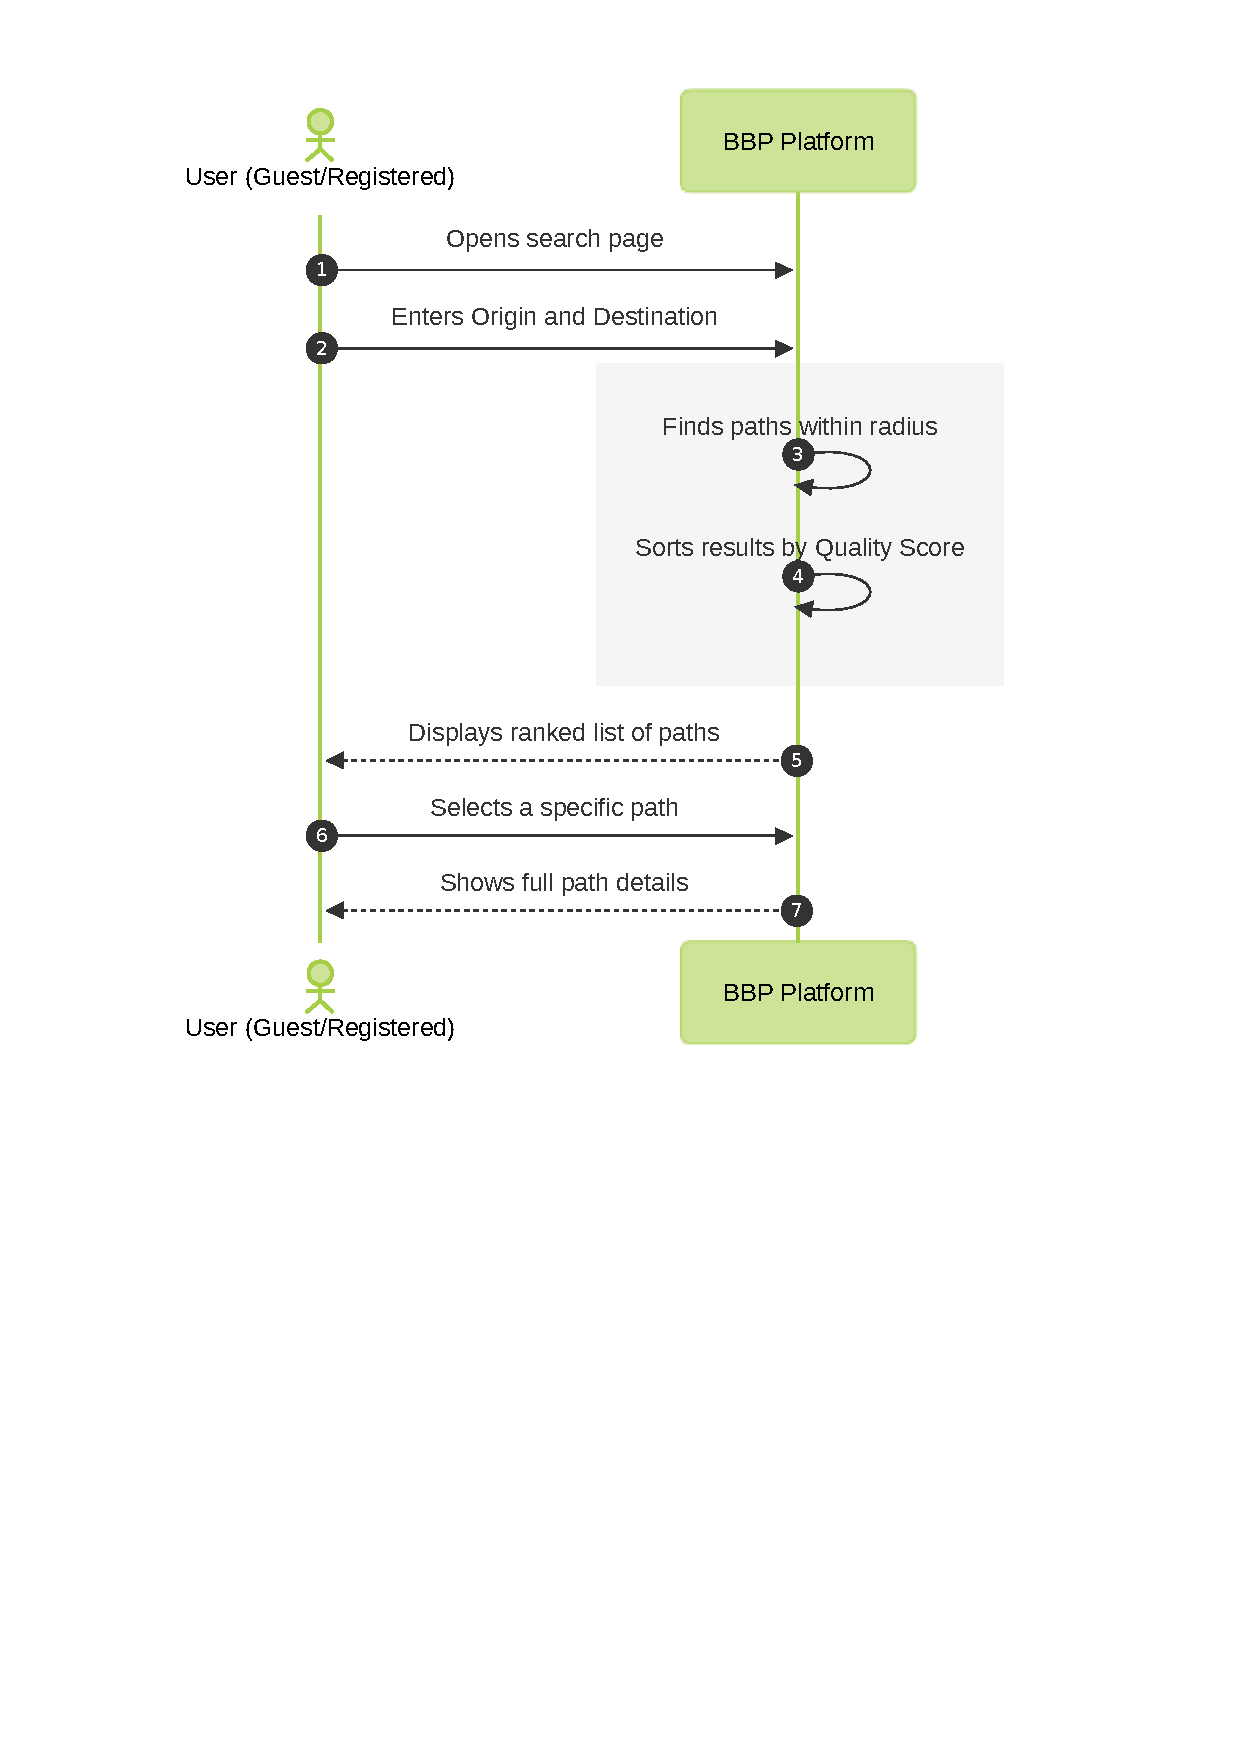
\includegraphics[width=\linewidth]{RASD/images/uc03.pdf}
    \caption{Search of Bike Paths}
    \label{fig:uc3}
\end{figure}

\begin{figure}[h!]
    \centering
    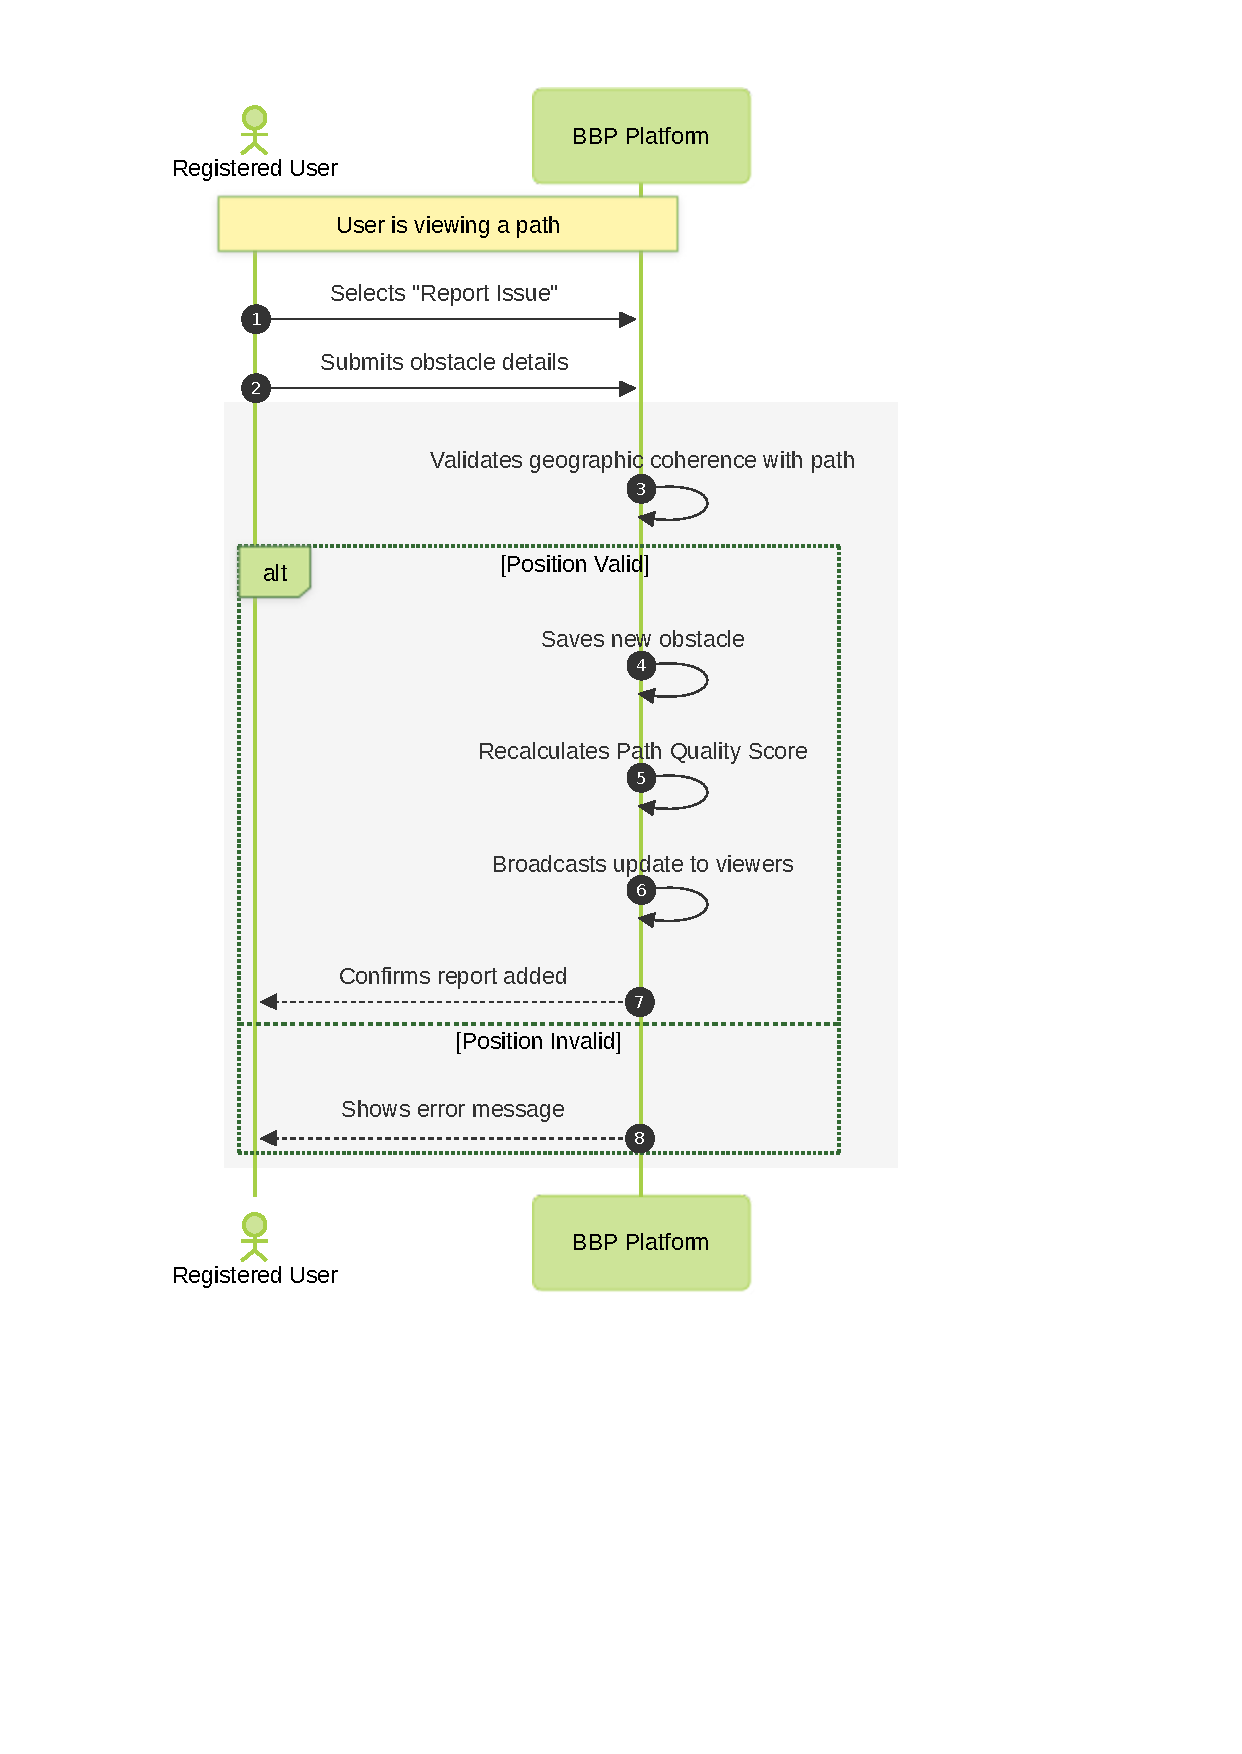
\includegraphics[width=\linewidth]{RASD/images/uc04.pdf}
    \caption{Obstacle Reporting on Bike Path}
    \label{fig:uc4}
\end{figure}

\begin{figure}[h!]
    \centering
    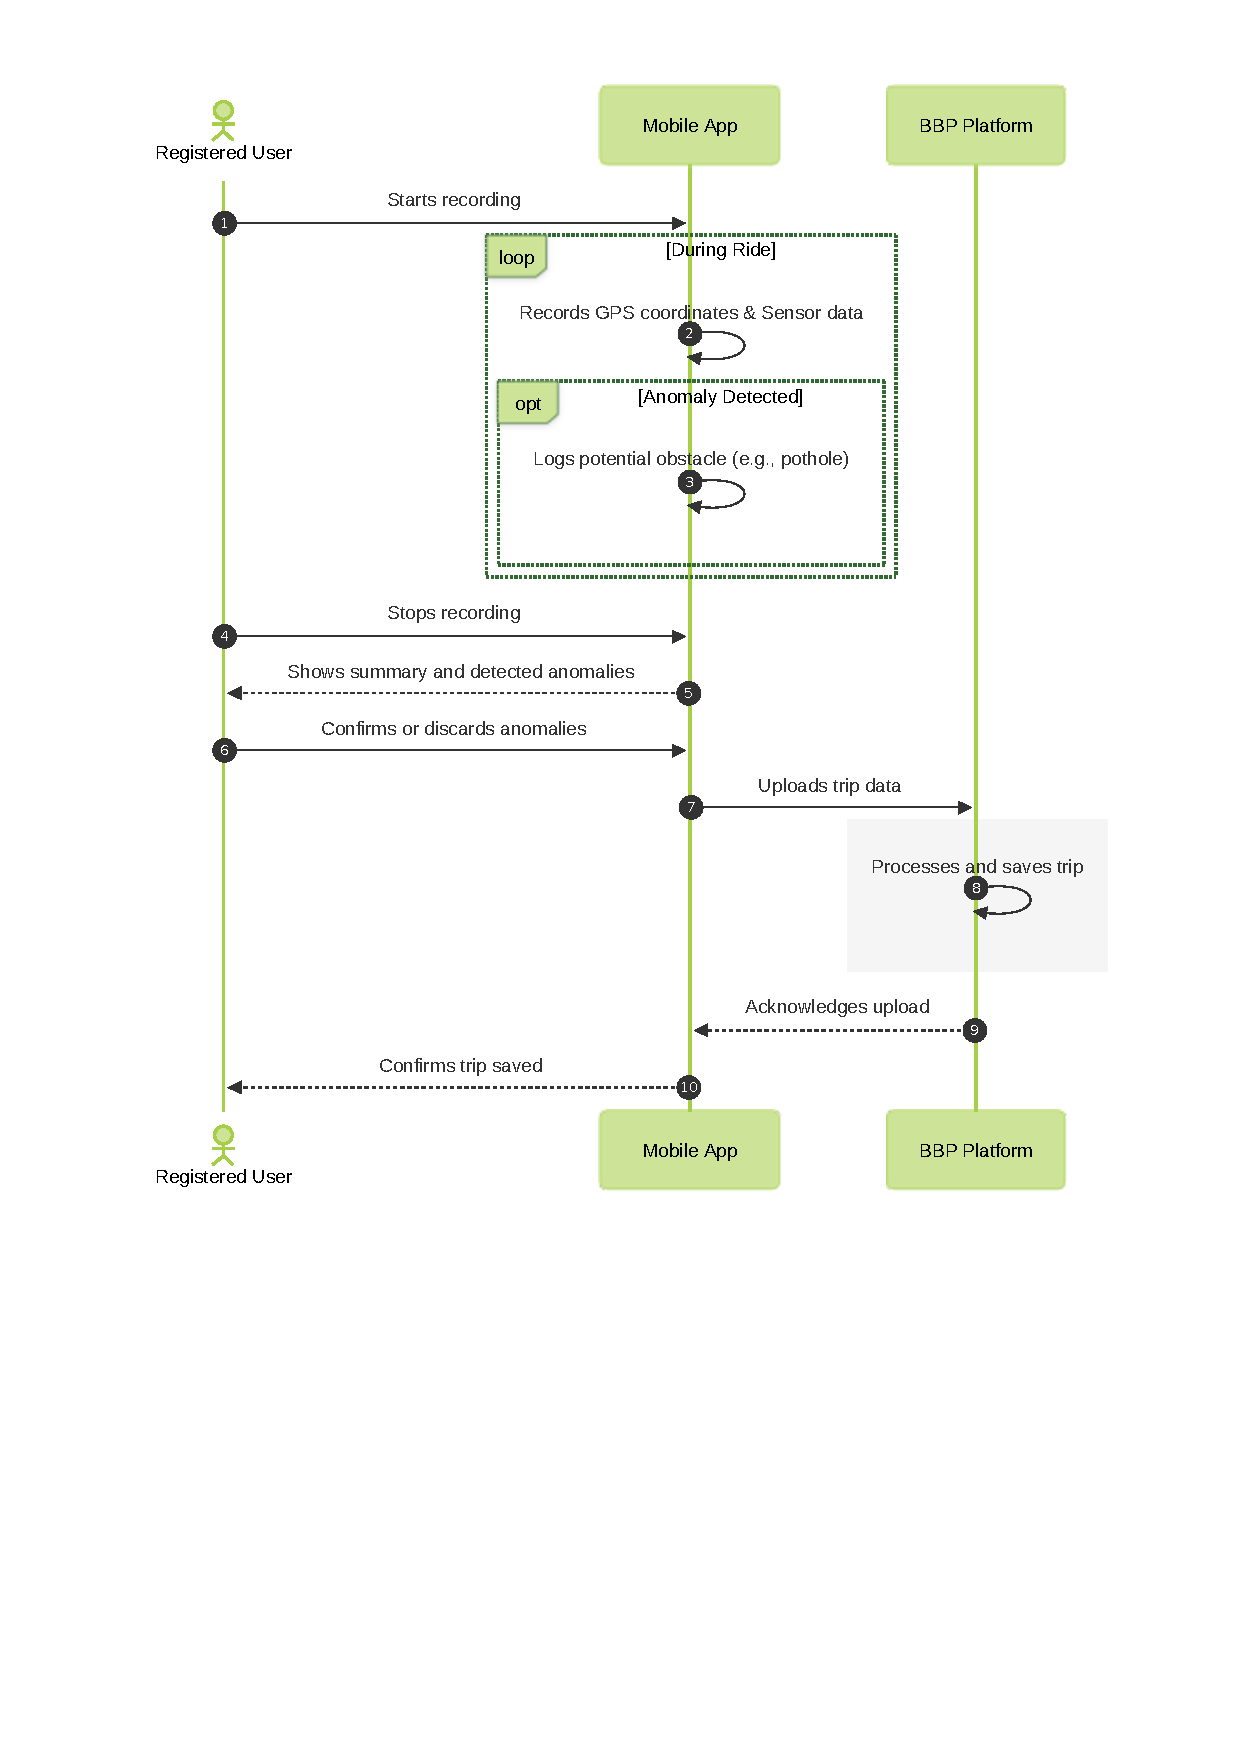
\includegraphics[width=\linewidth]{RASD/images/uc05.pdf}
    \caption{Automatic Tracking}
    \label{fig:uc5}
\end{figure}

\begin{figure}[h!]
    \centering
    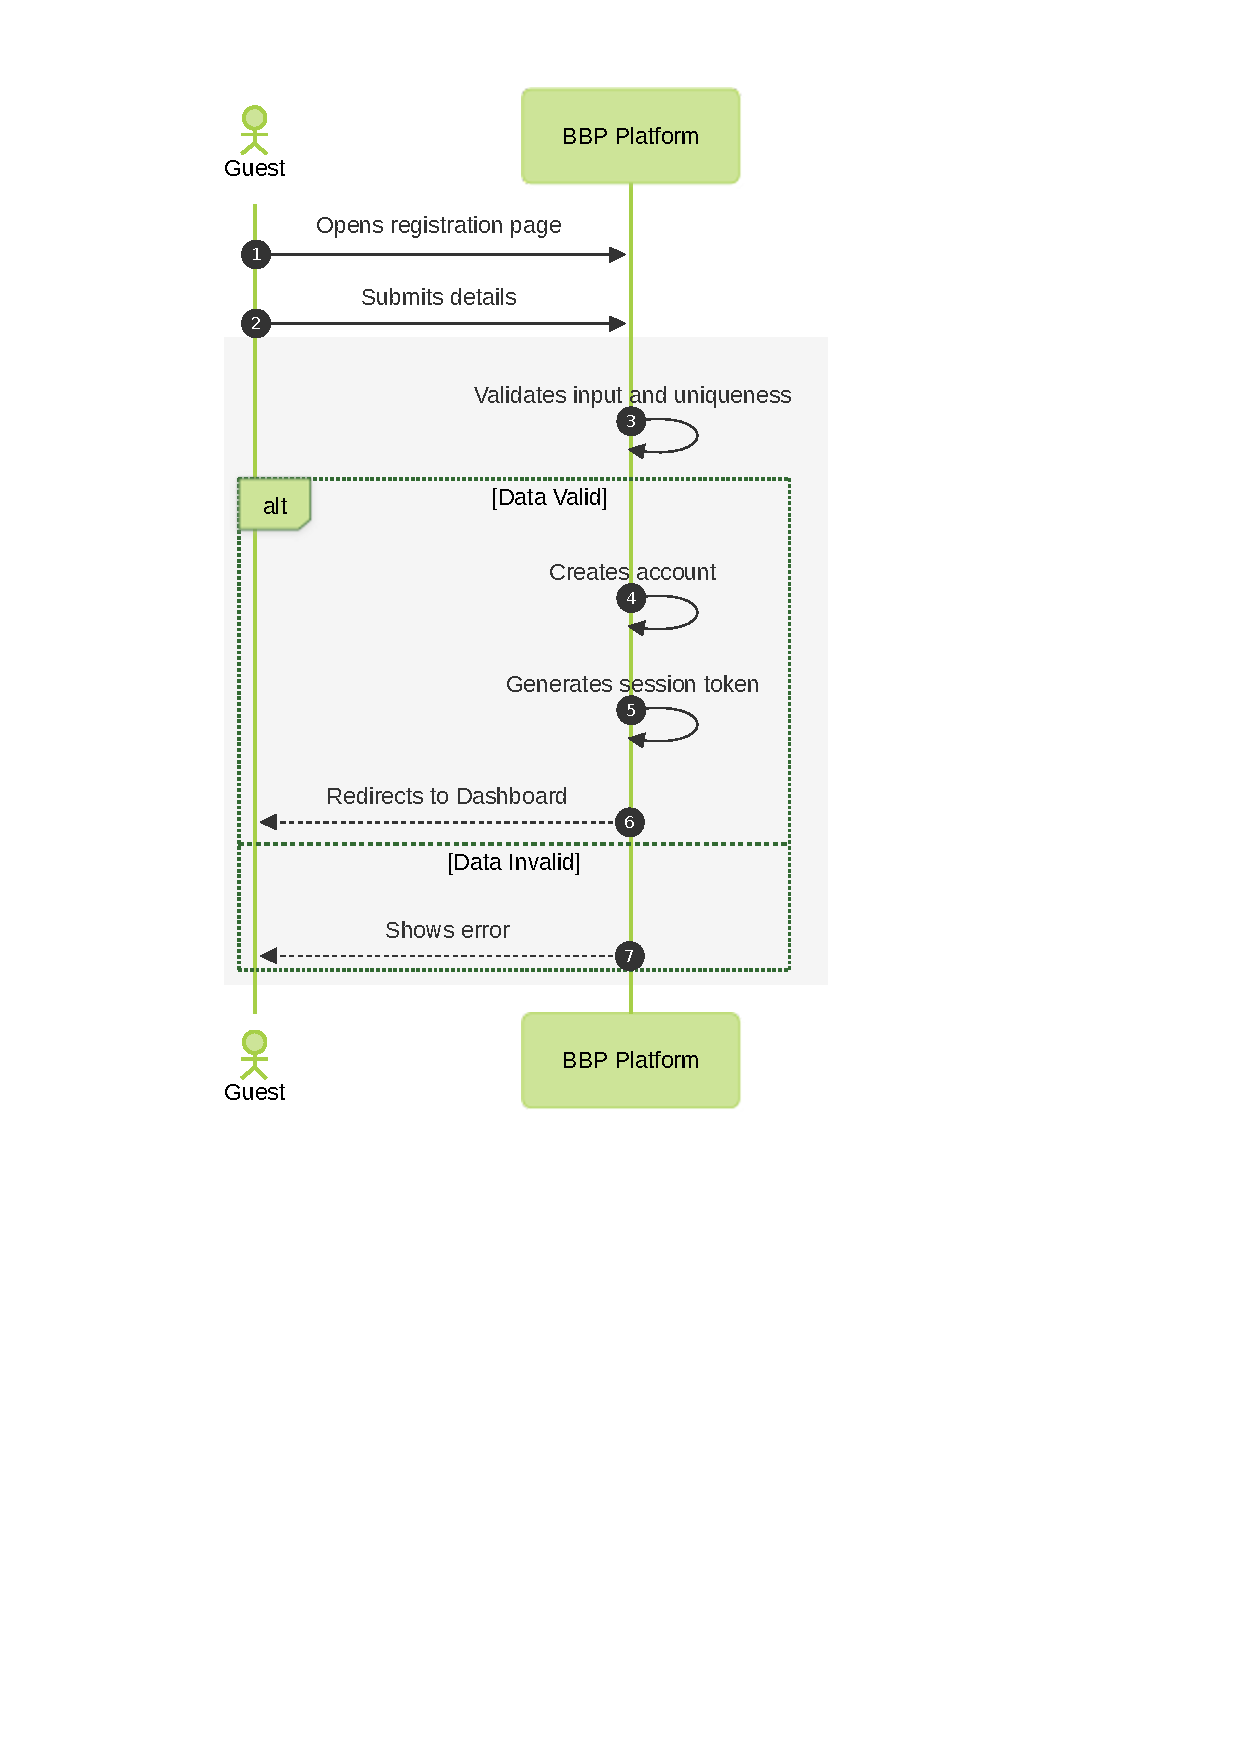
\includegraphics[width=\linewidth]{RASD/images/uc06.pdf}
    \caption{User Registration}
    \label{fig:uc6}
\end{figure}

\begin{figure}[h!]
    \centering
    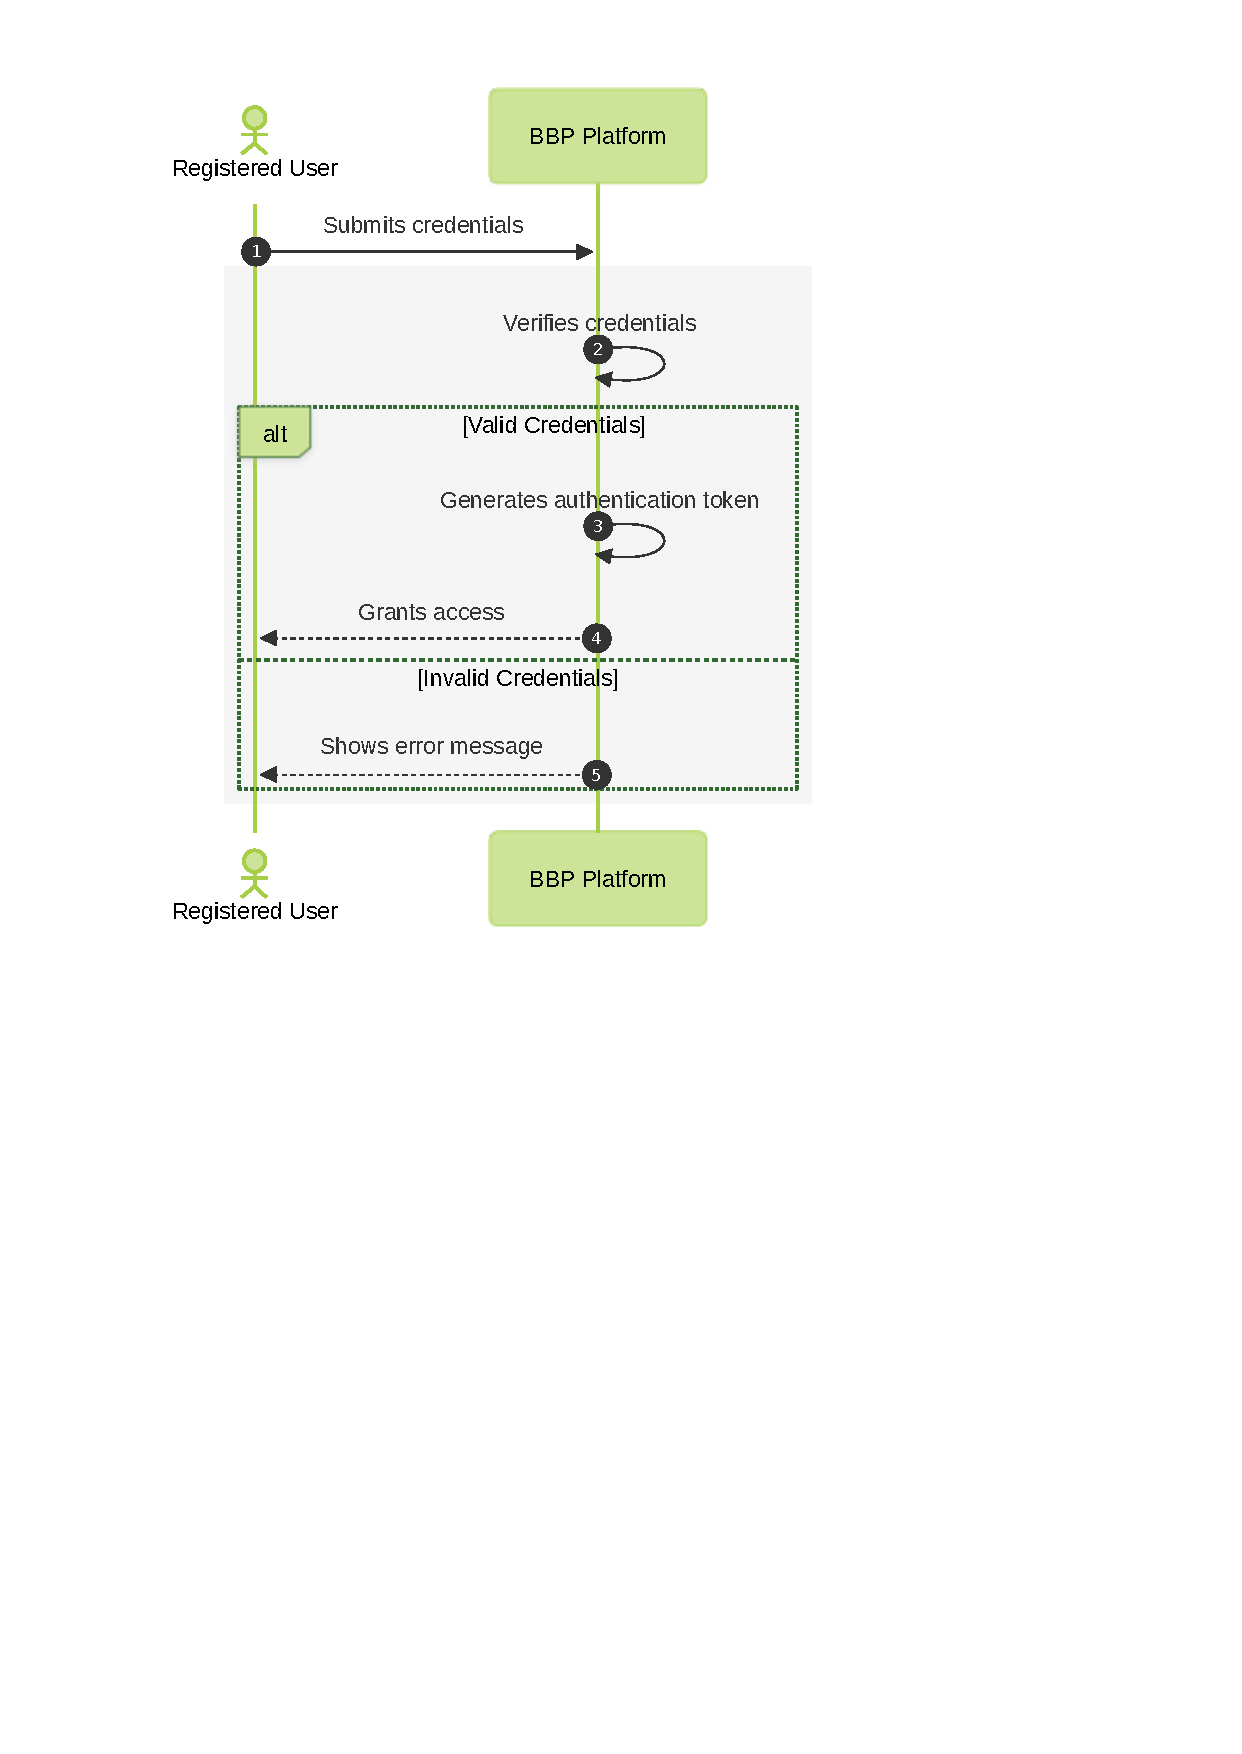
\includegraphics[width=\linewidth]{RASD/images/uc07.pdf}
    \caption{User Login}
    \label{fig:uc7}
\end{figure}

\begin{figure}[h!]
    \centering
    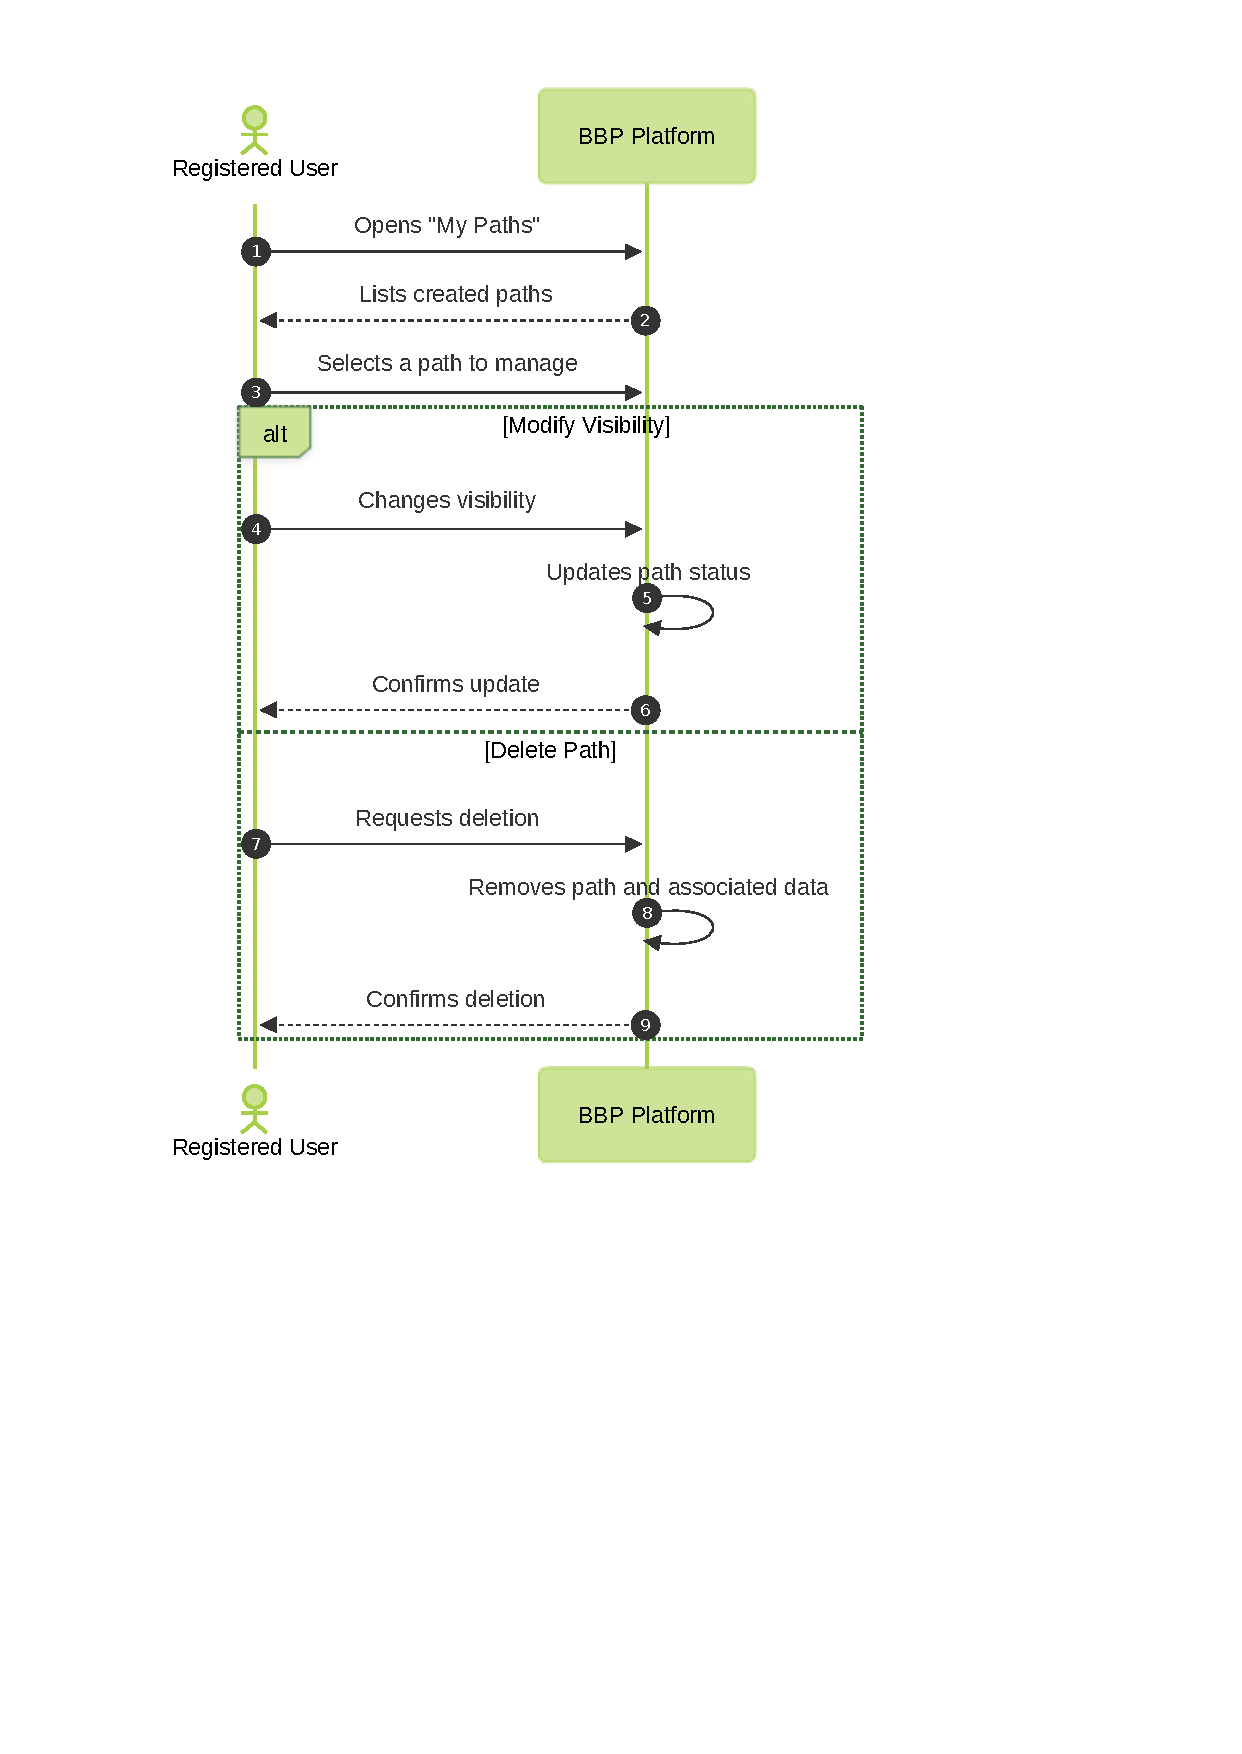
\includegraphics[width=\linewidth]{RASD/images/uc08.pdf}
    \caption{Management of Created Bike Paths}
    \label{fig:uc8}
\end{figure}

\begin{figure}[h!]
    \centering
    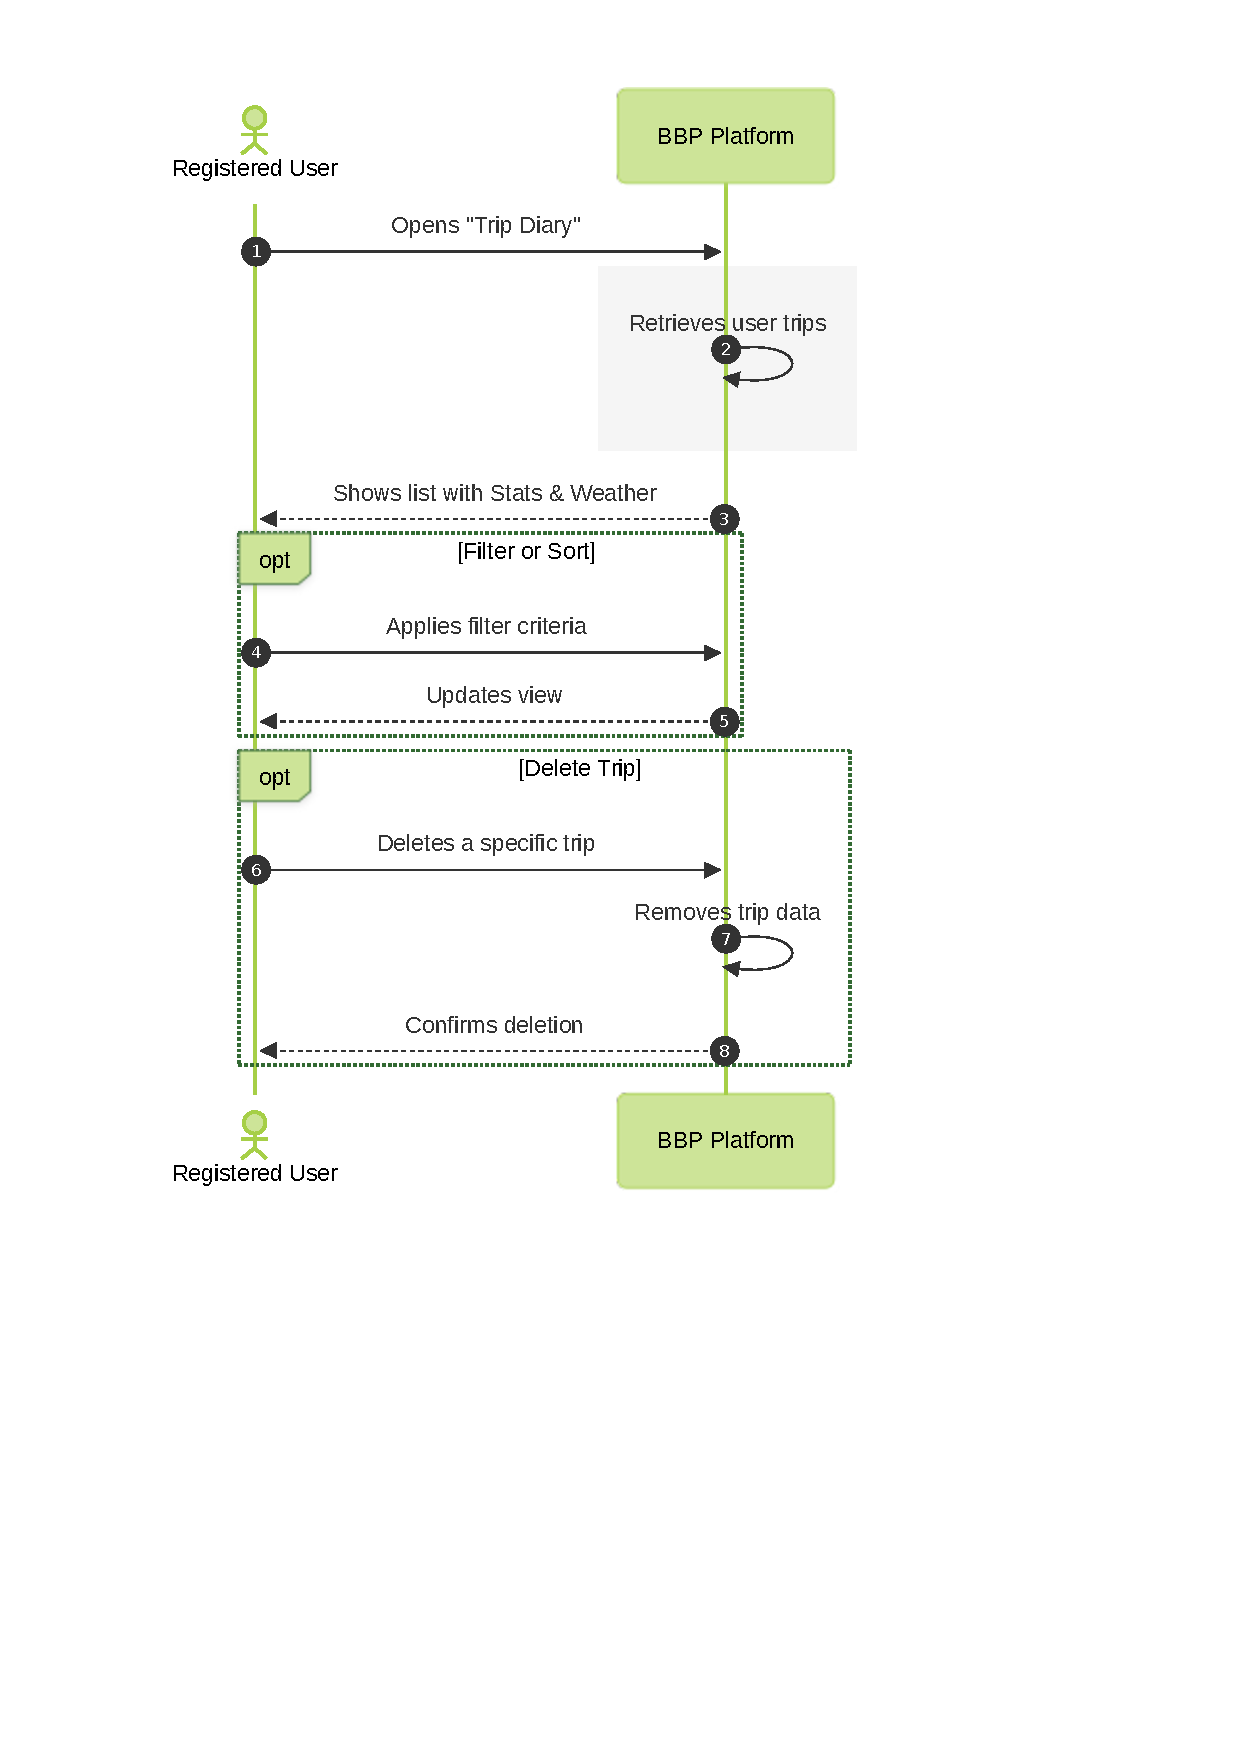
\includegraphics[width=\linewidth]{RASD/images/uc09.pdf}
    \caption{Trip History Visualization and Management}
    \label{fig:uc9}
\end{figure}

\begin{figure}[h!]
    \centering
    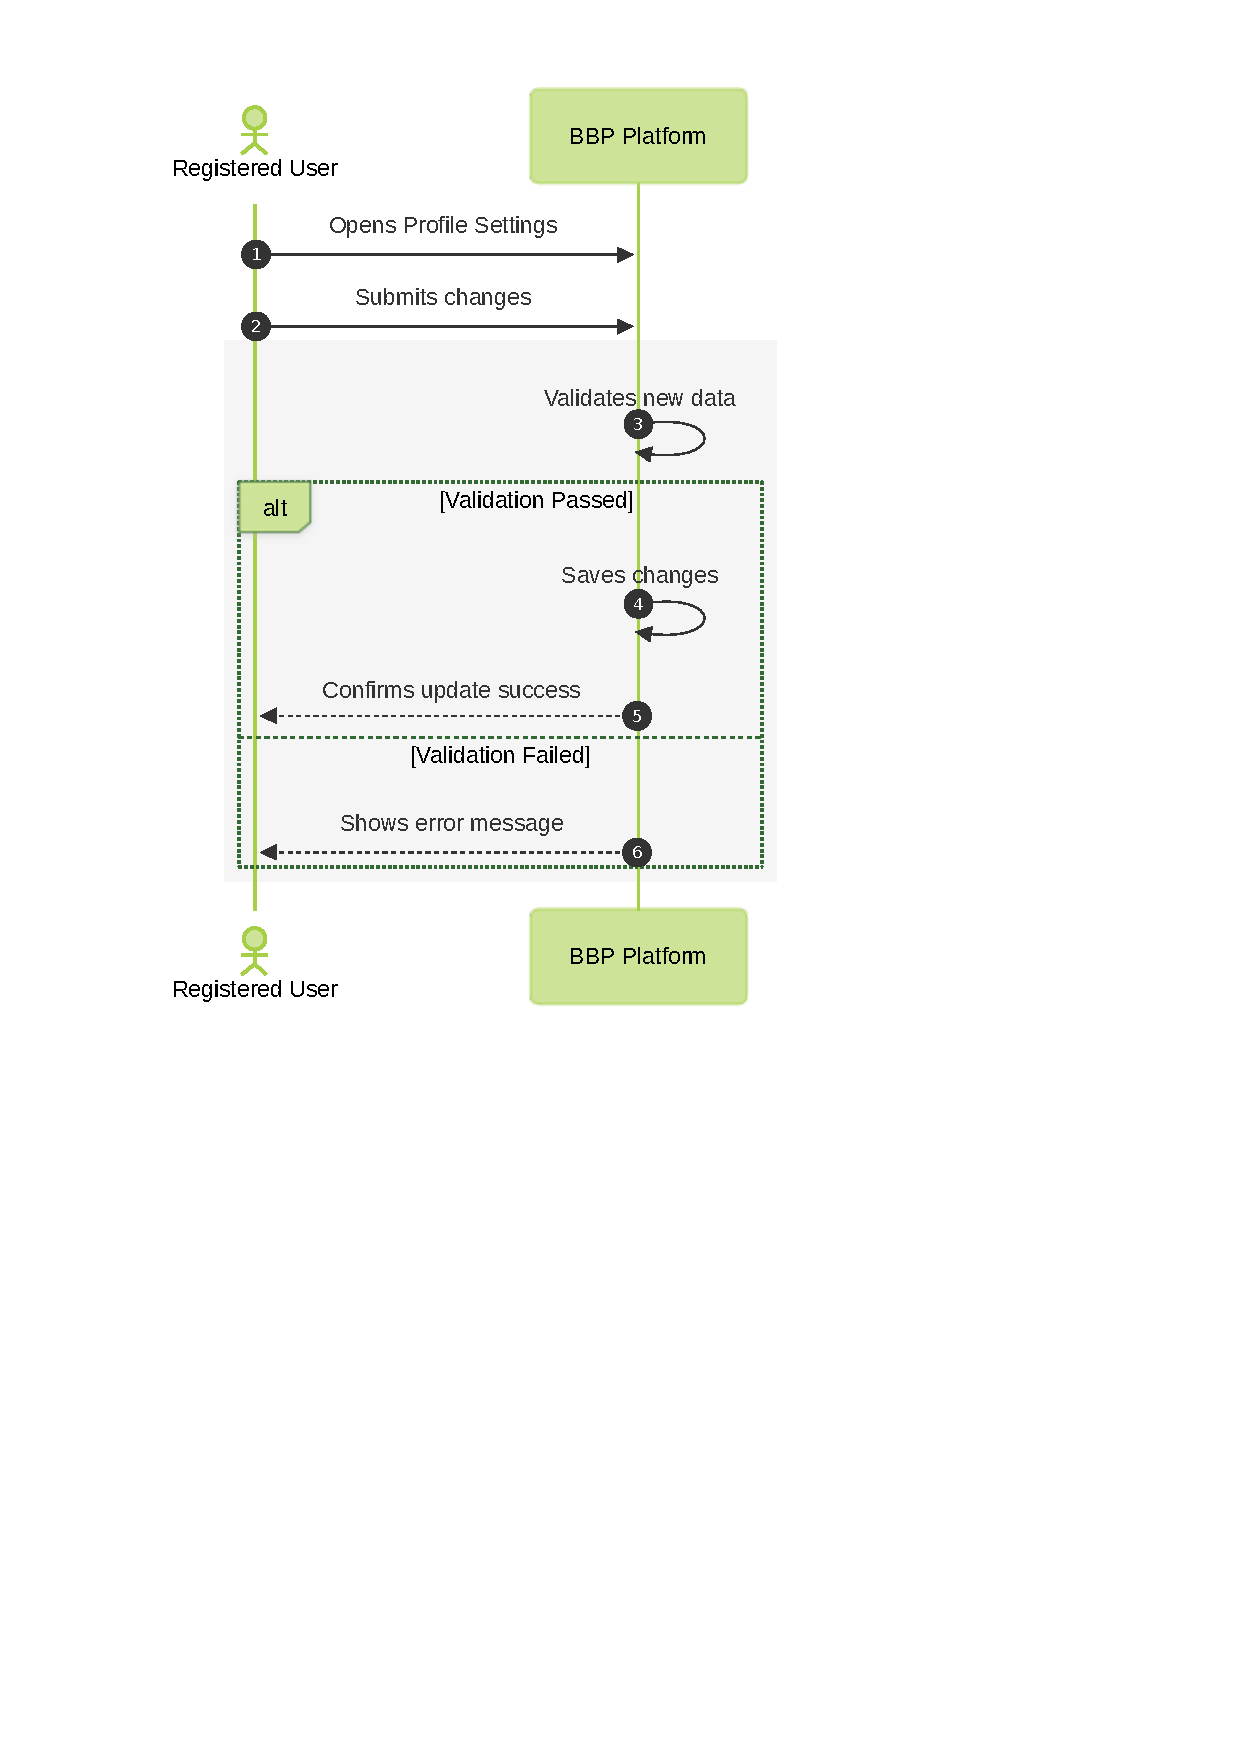
\includegraphics[width=\linewidth]{RASD/images/uc10.pdf}
    \caption{User Profile Update}
    \label{fig:uc10}
\end{figure}

\clearpage

\subsubsection{Requirement Mapping}

\begin{table}[H]
    \centering
    \begin{tabular}{|p{7cm}|p{7cm}|}
        \hline
        \multicolumn{2}{|p{14cm}|}{\textbf{[G1]} Planning best and most efficient bike path} \\
        \hline
        \textbf{Requirements} & \textbf{Domain Assumptions} \\
        \hline
        \textbf{[R19]} The system allows any user to search for public bike paths within a specific geographic radius between an origin and a destination. \newline
        \textbf{[R20]} The system shows search results sorted by descending Quality Score. \newline
        \textbf{[R16]} The system automatically calculates a Quality Score based on status and obstacles. & 
        \textbf{[D3]} Users have a working stable internet connection. \newline
        \textbf{[D6]} External services (Map providers) maintain their standard service levels. \newline
        \textbf{[D9]} Geocoding and routing data provided by map services are accurate and up-to-date. \\
        \hline
    \end{tabular}
    \caption{Mapping for G1}
    \label{tab:map_g1}
\end{table}

\begin{table}[H]
    \centering
    \begin{tabular}{|p{7cm}|p{7cm}|}
        \hline
        \multicolumn{2}{|p{14cm}|}{\textbf{[G2]} Storing the cycling activity of registered users} \\
        \hline
        \textbf{Requirements} & \textbf{Domain Assumptions} \\
        \hline
        \textbf{[R1]-[R4]} User registration, login, logout, and profile management. \newline
        \textbf{[R5]} Manual trip recording. \newline
        \textbf{[R6]} Automatic calculation of total distance and average speed. \newline
        \textbf{[R7]} Automatic enrichment with historical weather data. \newline
        \textbf{[R9]} Visualization of trip history and individual statistics. \newline
        \textbf{[R10]} Trip deletion. & 
        \textbf{[D3]} Users have a working stable internet connection. \newline
        \textbf{[D6]} External services maintain their standard service levels. \newline
        \textbf{[D8]} Historical weather conditions retrieved from external services are correct. \\
        \hline
    \end{tabular}
    \caption{Mapping for G2}
    \label{tab:map_g2}
\end{table}

\begin{table}[H]
    \centering
    \begin{tabular}{|p{7cm}|p{7cm}|}
        \hline
        \multicolumn{2}{|p{14cm}|}{\textbf{[G3]} Automatic cycling activity recognizer and recorder} \\
        \hline
        \textbf{Requirements} & \textbf{Domain Assumptions} \\
        \hline
        \textbf{[R8]} The system allows users to automatically track trips in real-time via GPS. \newline
        \textbf{[R12]} The system allows users to automatically record bike paths through GPS tracking and sensor data. & 
        \textbf{[D1]} Users own smartphones with working GPS, accelerometer, and gyroscope. \newline
        \textbf{[D2]} The user's phone has enough battery to sustain continuous sensor usage. \newline
        \textbf{[D4]} GPS accuracy is sufficient. \newline
        \textbf{[D7]} Users' riding behavior respects typical cycling patterns. \\
        \hline
    \end{tabular}
    \caption{Mapping for G3}
    \label{tab:map_g3}
\end{table}

\begin{table}[H]
    \centering
    \begin{tabular}{|p{7cm}|p{7cm}|}
        \hline
        \multicolumn{2}{|p{14cm}|}{\textbf{[G4]} Automatically detect cycling stop and verify gathered data} \\
        \hline
        \textbf{Requirements} & \textbf{Domain Assumptions} \\
        \hline
        \textbf{[R8]} The system detects stop and displays a trip summary for user confirmation. \newline
        \textbf{[R12]} The system detects stop, displays a summary with detected obstacles, and requests user validation before saving the bike path. & 
        \textbf{[D5]} Users provide truthful and accurate feedback during manual validation of automatically collected data. \\
        \hline
    \end{tabular}
    \caption{Mapping for G4}
    \label{tab:map_g4}
\end{table}

\begin{table}[H]
    \centering
    \begin{tabular}{|p{7cm}|p{7cm}|}
        \hline
        \multicolumn{2}{|p{14cm}|}{\textbf{[G5]} Permitting manual insertions} \\
        \hline
        \textbf{Requirements} & \textbf{Domain Assumptions} \\
        \hline
        \textbf{[R5]} Manual trip recording with streets and timings. \newline
        \textbf{[R11]} Creation of new bike paths by specifying origin, destination, and streets. \newline
        \textbf{[R13]} Automatic calculation of path geometry and length. \newline
        \textbf{[R14]} Manual addition of obstacles to bike paths with type and severity. \newline
        \textbf{[R15]} Validation of obstacle location within path buffer. & 
        \textbf{[D3]} Users have a working stable internet connection. \newline
        \textbf{[D5]} Users provide truthful and accurate feedback during manual entry. \newline
        \textbf{[D6]} External map services function correctly for geocoding and routing. \newline
        \textbf{[D9]} Geocoding and routing data provided by map services are accurate and up-to-date. \\
        \hline
    \end{tabular}
    \caption{Mapping for G5}
    \label{tab:map_g5}
\end{table}

\begin{table}[H]
    \centering
    \begin{tabular}{|p{7cm}|p{7cm}|}
        \hline
        \multicolumn{2}{|p{14cm}|}{\textbf{[G6]} Publication control} \\
        \hline
        \textbf{Requirements} & \textbf{Domain Assumptions} \\
        \hline
        \textbf{[R17]} The system allows the creator of a bike path to manage its visibility (private or public). & 
        \textbf{[D5]} Users make informed decisions about data sharing. \\
        \hline
    \end{tabular}
    \caption{Mapping for G6}
    \label{tab:map_g6}
\end{table}

\subsection{Performance Requirements}

The system must be able to handle a high volume of telemetry data sent in real-time by users' mobile phones during biking activities, guaranteeing the necessary scalability to handle thousands of concurrent connections without system degradation.
Given the nature of the mobile app, it is fundamental that mobile phones' resources are optimized to keep the battery consumption at an acceptable rate during long activities.
Moreover, the system must guarantee fast response times for route calculation and map rendering, ensuring smooth and responsive navigation even in suboptimal connectivity conditions. The system must propagate updates to road quality and obstacle presence to all clients quickly enough to prevent any client from viewing outdated data.

\subsection{Design Constraints}

\subsubsection{Standards Compliance}
\begin{itemize}
    \item[] \textbf{GDPR \& Privacy:} The system gathers sensitive and private data such as emails, passwords, and users' GPS coordinates. System development and data handling must be compliant with GDPR regulations. In particular, users' personal tracks must be kept private unless the user explicitly chooses to make them public.
    
    \item[] \textbf{Data Security:} Users' credentials must be protected through secure password hashing algorithms. All client-server communications must be encrypted using TLS/SSL protocols to ensure confidentiality and integrity of transmitted data.
\end{itemize}

\subsubsection{Hardware Limitations}
\begin{itemize}
    \item[] \textbf{Device Sensors:} The mobile app requires specific hardware components for automatic tracking functionality (GPS module, accelerometer, and gyroscope). In the absence of these sensors, the automatic tracking and obstacle detection features are unavailable.
    
    \item[] \textbf{Mobile Devices:} The UI and mobile app must be optimized to run efficiently on most modern devices without causing device overheating or excessive battery drain.
\end{itemize}

\subsubsection{Other Constraints}
\begin{itemize}
    \item[] \textbf{Connectivity:} The app must be designed considering that users' internet connections may be unstable during cycling sessions in remote areas. The system must include local caching mechanisms for essential data such as route information and recent bike path details.
    
    \item[] \textbf{External Dependencies:} The system depends on third-party services for maps and weather data. The design must comply with the API usage limits, rate limiting, and terms of service of the external service providers.
\end{itemize}

\subsection{Software System Attributes}

\subsubsection{Reliability} 
The system must preserve important information gathered by users. The database must be replicated across several nodes and regularly backed up in order to prevent data loss in the event of server-side hardware failures.
Reliability on the client side implies the ability to prevent data loss from the live tracking session, even in the case of an application crash or abrupt device shutdown; the system must incorporate mechanisms for frequent local checkpointing.


\subsubsection{Availability} 
The BBP system must ensure a high level of availability, especially during expected peak periods, guaranteeing a target uptime of \textbf{99\%}. 
The architecture must incorporate redundancy and failover mechanisms for core services. In the event of external service unavailability, the system must gracefully degrade functionality without interrupting the core service.
 
\subsubsection{Security} 
BBP handles user credentials that must be stored using robust hashing algorithms. All data in transit between mobile apps, web apps, and servers must be encrypted using secure protocols. 
The system must implement active defenses against common web vulnerabilities.

\subsubsection{Maintenance}
The system must use a modular architecture that clearly divides business logic, user interface, and data processing to enable future software evolution.
The backend's exposed APIs must be clearly defined and versioned to enable server updates without affecting compatibility with earlier iterations of the mobile application.

\subsubsection{Portability}
Regardless of the desktop operating system being used, the system's web component must work with all of the major modern browsers.
In order to provide a consistent user experience across a variety of devices, the mobile application must be made to be portable between the most common mobile operating systems.